\documentclass[11pt,a4paper]{article}
\usepackage[T1]{fontenc}
\usepackage[utf8]{inputenc}
\usepackage{lmodern}
\usepackage[margin=27mm,headheight=14pt]{geometry}
\usepackage{amsmath,amssymb,amsthm,mathtools,bm}
\usepackage{microtype,booktabs,longtable,array,enumitem}
\usepackage{xcolor,graphicx,fancyhdr}
\usepackage[section]{placeins}
\usepackage[hyphens]{url}
\usepackage[colorlinks=true,linkcolor=blue!45!black,citecolor=blue!45!black,urlcolor=blue!55!black]{hyperref}
\usepackage[nameinlink,noabbrev]{cleveref}
\numberwithin{equation}{section}
\newtheorem{theorem}{Theorem}[section]
\newtheorem{proposition}[theorem]{Proposition}
\newtheorem{lemma}[theorem]{Lemma}
\newtheorem{corollary}[theorem]{Corollary}
\newtheorem{conjecture}[theorem]{Conjecture}
\theoremstyle{definition}
\newtheorem{definition}[theorem]{Definition}
\newtheorem{example}[theorem]{Example}
\theoremstyle{remark}
\newtheorem{remark}[theorem]{Remark}
\newcommand{\Li}{\operatorname{Li}}
\newcommand{\Rea}{\operatorname{Re}}
\newcommand{\Ima}{\operatorname{Im}}
\newcommand{\dd}{\,\mathrm d}
\newcommand{\ii}{\mathrm i}
\newcommand{\E}{\mathbb E}
\newcommand{\R}{\mathbb R}
\newcommand{\C}{\mathbb C}
\newcommand{\Q}{\mathbb Q}
\newcommand{\D}{\mathcal D}
\newcommand{\mesh}{\operatorname{mesh}}
\newcommand{\supp}{\operatorname{supp}}
\newcommand{\sgn}{\operatorname{sgn}}
\newcommand{\eps}{\varepsilon}
\newcommand{\Res}{\operatorname{Res}}
\newcommand{\FP}{\operatorname{FP}}
\setlist{itemsep=3pt,topsep=5pt}
\setlength{\emergencystretch}{2em}
\pagestyle{fancy}
\fancyhf{}
\fancyhead[L]{\small Polylogarithms: extremizers, zeros, and identities}
\fancyhead[R]{\small ProveIt continuation}
\fancyfoot[C]{\thepage}
\hypersetup{pdftitle={Polylogarithms: Global Euler Extremizers, Polynomial Zero Thresholds, and Mixed Gaussian Identities},pdfauthor={ProveIt research continuation},pdfsubject={Rigorous continuation at revision 4c173c06cc32c9cea554b39be1837ad2ae897fc1}}
\title{\textbf{Polylogarithms: Global Euler Extremizers,\\Polynomial Zero Thresholds,\\and Mixed Gaussian Identities}}
\author{A research continuation for the ProveIt project}
\date{10 October 2026}
\begin{document}
\maketitle
\begin{abstract}
This article continues the polylogarithm programme at the immutable
ProveIt revision \texttt{4c173c06cc32c9cea554b39be1837ad2ae897fc1},
including the six archives present in its incoming directory. The emphasis
is on precise outstanding extremal and zero-separation questions, with
complete ordinary proofs and reproducible finite calculations. We prove
the global scaling conjecture for the positive Euler remainder kernel,
describe its eventual unique maximizer by a convergent expansion, and
give an exact degree-seven characterization at truncation two.
For the optimal order-averaged remainder we prove eventual exact
reduction to the outer-order axis, settle the conjectured leading
power law, and find a second scale of order
$N^{-1.9695904\ldots}/\sqrt{\log N}$.
A polynomial lower bound $\mesh(Q_n)\ge1/(10n^2)$ for reciprocal-gamma
Appell roots yields a uniform Lerch zero threshold of order
$n^4\log^2 n$ and a growing-index range of order
$k^{1/4}/\sqrt{\log k}$.
We classify the complete Gaussian sign transitions at outer orders
$-2$ and $-3$, prove cyclotomic sampling and elementary resummation
identities for the mixed Gaussian generator, and propose a weight-fifteen
relation with an exact rational residual bound below $10^{-775}$.
The last equality remains conjectural. An audit, integration notes,
and fourteen research questions specify the remaining work.
\end{abstract}

\vfill
\noindent\small
\textbf{Source snapshot.} ProveIt revision
\texttt{4c173c06cc32c9cea554b39be1837ad2ae897fc1}, including all six
incoming archives present on 10 October 2026. Complete TeX sources,
exact certificates, numerical diagnostics, and integration notes
accompany this article.\normalsize
\clearpage
\tableofcontents
\clearpage
\section{Scope, conventions, and the questions being continued}
\label{sec:intro}
The canonical manuscript at the stated revision is a 379-page synthesis;
its six incoming archives contain further overlapping continuations
\cite{ProveIt,IncomingSharp,IncomingBounds,IncomingUniform,IncomingMixed,
IncomingRadial,IncomingDepth}. In particular, the $S_4$ Gaussian identity,
the three recorded golden-ratio weight-five formulas, and the sharp
Euler constant uniform in all positive orders have already been proved.
They are background here. The existing $S_6$ and higher mixed Gaussian
evaluations must still be assessed within their stated relation systems.

Our first point of departure is the positive remainder kernel
\begin{equation}\label{eq:intro-kernel}
 f_N(v)=\frac{(1-v)^N}{1+v},\qquad
 K_N(p,y)=\frac{f_N(py^2)-f_N(p)}{1-y},\qquad 0\le p,y\le1.
\end{equation}
The quotient uses its continuous value at $y=1$.
The archive \cite[Section 8]{IncomingSharp} conjectures convergence of
its global maxima to an exponential limiting kernel. A local scaling
limit had been proved there; the missing global compactness argument
and uniqueness of the limit are supplied below. Its finite-index
uniqueness and monotonicity conjecture receives an exact answer at
$N=2$ and an eventual answer for large $N$.

The second point of departure is the zero geometry of the Stieltjes--Lerch
derivative family. Its Laplace representation uses the Appell polynomials
\[
 \frac{e^{xz}}{\Gamma(1+z)}
   =\sum_{n\ge0}Q_n(x)\frac{z^n}{n!}.
\]
The effective incoming theorem \cite[Section 4]{IncomingUniform}
uses an exponentially small lower bound on their root separation.
Replacing that bound by a polynomial estimate changes the permitted
growth of the Laurent index substantially.

Throughout, a multiple polylogarithm has decreasing summation indices:
\[
 \Li_{a,b}(z,w)=\sum_{n>m\ge1}\frac{z^nw^m}{n^am^b}
\]
in its domain of absolute convergence, followed by the specified analytic
continuation. Put
\begin{equation}\label{eq:F-def}
 F_{a,b}(z)=\Li_{a,b}(z,1)
   =\sum_{n\ge1}\frac{H_{n-1}^{(b)}}{n^a}z^n,
 \qquad H_m^{(b)}=\sum_{j=1}^m j^{-b},\qquad
 g_{a,b}=\Ima F_{a,b}(\ii).
\end{equation}
For $a\ge0,b>0$ we use the principal continuation on
$\C\setminus[1,\infty)$. Negative integer outer orders are obtained
by powers of $\D=z\,\mathrm d/\mathrm dz$. The Dirichlet functions are
\[
 \beta(s)=\sum_{m\ge0}\frac{(-1)^m}{(2m+1)^s},\qquad
 \eta(s)=\sum_{m\ge1}\frac{(-1)^{m-1}}{m^s}
\]
where these series converge, and their analytic continuations elsewhere.
Our logarithms of positive real quantities are real logarithms.

\paragraph{Status of the mathematics.}
All statements marked theorem, proposition, lemma, or corollary are
proved in this article, with any inherited input explicitly identified
and justified as needed. The higher-weight relation marked conjecture
has a frozen coefficient vector and an exact rational residual enclosure;
an enclosure containing zero is not a proof of equality. None of the
ordinary proofs or finite replay scripts is a proof-assistant
formalization. The claims of advancement refer to the audited repository
snapshot, not to an exhaustive assertion of priority over the literature.

\clearpage
\section{Global extrema of the Euler remainder kernel}
\label{sec:kernel}

\subsection{Why this kernel occurs}
For $a,b>0$, let $S_a,T_b$ be independent gamma variables of shapes
$a,b$ and rate one, and put $X=e^{-S_a}$, $Y=e^{-T_b}$.
At $a=0$, take $X=1$. Their moments are
\[
 \E X^{n-1}=n^{-a},\qquad \E Y^{m-1}=m^{-b}.
\]
Writing the inner harmonic number as a geometric sum proves
\begin{equation}\label{ker:eq:continuation}
 F_{a,b}(z)=z^2\E\frac{X}{(1-zX)(1-zXY)}.
\end{equation}
Initially this follows by absolute convergence in the disk. On compact
subsets of the principal slit plane, both denominators have positive
uniform lower bounds, so the expectation is holomorphic and proves
continuation. In particular,
\[
 g_{a,b}=-\E\frac{X^2(1+Y)}{(1+X^2)(1+X^2Y^2)}<0.
\]

Define the finite Euler approximants by
\begin{equation}\label{ker:eq:euler}
 A_j=\frac{H_{2j}^{(b)}}{(2j+1)^a},\qquad
 d_j=\sum_{m=0}^j(-1)^m\binom jm A_m,
 \qquad E_N=\sum_{j=0}^{N-1}\frac{d_j}{2^{j+1}}.
\end{equation}
The classical transformation and forward-difference convention are
recorded in \cite[Section 3.9(ii)]{DLMF}. Here the finite geometric
identity gives an exact analytic remainder, even when the original
boundary series is not convergent:
\begin{equation}\label{ker:eq:remainder}
 R_N(a,b):=2^N(E_N-g_{a,b})=\E K_N(X^2,Y)>0.
\end{equation}
Indeed,
\[
 d_j=\E\frac{(1-X^2)^j-(1-X^2Y^2)^j}{1-Y},
\]
and summing the finite geometric series proves
\eqref{ker:eq:remainder}. These steps retain the cancellation at $Y=1$;
they do not separate two divergent integrals.

The existing sharp bound uniform in all $a,b,N$ is inherited from
\cite{ProveIt,IncomingSharp,IncomingBounds}. Our present problem is the
different, pointwise optimization
\begin{equation}\label{ker:eq:MN}
 M_N=\max_{(p,y)\in[0,1]^2}K_N(p,y).
\end{equation}
An arbitrary maximizing point $(p,y)$ need not be realized by the gamma
family in \eqref{ker:eq:remainder}. Thus $M_N$ and the order-averaged
constant studied in the next section are distinct extremal problems.

\subsection{A uniform envelope and its limit}
For $m\ge2$, put
\[
 J_m(p,y)=\frac{(1-py^2)^m-(1-p)^m}{1-y}.
\]
Differentiation in $p$ shows that its unique interior maximum for
$0<y<1$ is attained at
\[
 p_m(y)=\frac{1-y^{2/(m-1)}}{1-y^{2m/(m-1)}}.
\]
Substitution gives the envelope
\begin{equation}\label{ker:eq:BN}
 J_m(p,y)\le B_m(y):=(1+y)
 \left(\frac{1-y^2}{1-y^{2m/(m-1)}}\right)^{m-1}.
\end{equation}
The boundary values are $B_m(0)=1$ and
$B_m(1)=2((m-1)/m)^{m-1}$.
Moreover,
\begin{equation}\label{ker:eq:mixture}
 K_N(p,y)=\sum_{j\ge0}2^{-j-1}J_{N+j}(p,y).
\end{equation}
This follows from the geometric expansion of $(1+v)^{-1}$ in powers
of $1-v$. At $y=1$ it follows by differentiating that uniformly
convergent geometric expansion, or by continuity.

The envelope calculation and its monotonicity were proved in
\cite[Section 3]{IncomingSharp}. The following uniform quantitative
version supplies the global limiting argument.

\begin{lemma}[Uniform envelope convergence]\label{ker:lem:envelope}
Define
\begin{equation}\label{ker:eq:B}
 B(y)=(1+y)y^{2y^2/(1-y^2)}\quad(0<y<1),
 \qquad B(0)=1,\quad B(1)=2/e.
\end{equation}
For every $m\ge2$ and $0\le y\le1$,
\begin{equation}\label{ker:eq:uniform-envelope}
 B(y)\le B_m(y)\le B(y)\exp\!\left(\frac1{2(m-1)}\right).
\end{equation}
For $0<y<1$, $B_{m+1}(y)<B_m(y)$. Consequently
$K_N(p,y)\le B_N(y)$ for all $N\ge2$.
\end{lemma}
\begin{proof}
Set $t=-2\log y>0$, $k=m-1$, and
$h(v)=\log(1-e^{-(1+v)t})$. Then
\[
 \log B_m(y)=\log(1+y)-k\{h(1/k)-h(0)\},
 \qquad \log B(y)=\log(1+y)-h'(0).
\]
Here
\[
 h''(v)=-\left(\frac{t}{2\sinh((1+v)t/2)}\right)^2,
 \qquad -1\le h''(v)<0.
\]
Taylor's integral remainder therefore puts the difference of the two
logarithms between zero and $1/(2k)$. Concavity also shows that the
negative secant slope decreases as $k$ increases, giving strict
monotonicity. Continuity proves the endpoint inequalities.
Finally average \eqref{ker:eq:BN} in \eqref{ker:eq:mixture}.
\end{proof}

\begin{lemma}[The unique limiting maximum]\label{ker:lem:unique-limit}
The function $B$ has a unique global maximizer $y_\infty$ in $(0,1)$.
It is the unique root there of
\begin{equation}\label{ker:eq:Qroot}
 Q(y)=1+y-y^2-y^3+4y\log y=0.
\end{equation}
The maximum is nondegenerate. Put
\begin{equation}\label{ker:eq:limitconstants}
 c_\infty=\frac{-2\log y_\infty}{1-y_\infty^2}
           =\frac{1+y_\infty}{2y_\infty},\qquad
 M_\infty=(1+y_\infty)
      \exp\!\left(-\frac{y_\infty(1+y_\infty)}2\right).
\end{equation}
Then $M_\infty>1$, and
\[
 H(c,y)=\frac{e^{-cy^2}-e^{-c}}{1-y},\qquad
 H(c,1)=2ce^{-c},
\]
has the unique global maximizer $(c_\infty,y_\infty)$ on
$[0,\infty)\times[0,1]$. Its Hessian there is negative definite.
\end{lemma}
\begin{proof}
Differentiating $\log B$ gives
\[
 (\log B)'=\frac{Q(y)}{(1-y^2)^2},\qquad
 Q''(y)=-6y-2+\frac4y.
\]
The second derivative is positive on $(0,2/3)$ and negative on
$(2/3,1)$. Since $Q'(0+)=-\infty$ and $Q'(1)=0$, the derivative
$Q'$ has exactly one zero in $(0,2/3)$; it is negative before that
zero and positive after it, up to one. Also $Q(0+)=1$ and $Q(1)=0$.
Thus $Q$ crosses zero exactly once inside $(0,1)$, from positive to
negative, and $Q'(y_\infty)<0$. This proves uniqueness and
nondegeneracy of the maximum. Its value exceeds one, for example
because $B(1/4)>1$ is equivalent to the integer inequality
$5^{15}>2^{34}$.

For fixed $0<y<1$, differentiating $H$ in $c$ gives its unique maximum
at $c=-2\log y/(1-y^2)$, with value $B(y)$. At $y=0$ its supremum
is one, at $y=1$ its maximum is $2/e$, and at $c=0$ it is zero.
This proves the two-variable uniqueness. Equation \eqref{ker:eq:Qroot}
gives the second expression for $c_\infty$ in
\eqref{ker:eq:limitconstants}.
At a stationary point in $c$,
\[
 H_{cc}=-y^2(1+y)e^{-cy^2}<0.
\]
The Schur complement of this entry in the Hessian is the second
derivative of the optimized profile $B$, which is strictly negative
at $y_\infty$. Hence the Hessian is negative definite.
\end{proof}

\subsection{Resolution of the global limit conjecture}
\begin{theorem}[Global limiting extrema]\label{ker:thm:limit}
For every $N\ge2$,
\begin{equation}\label{ker:eq:two-sided}
 M_\infty<M_N\le M_\infty
                  \exp\!\left(\frac1{2(N-1)}\right).
\end{equation}
In particular, $M_N\to M_\infty$. If $(p_N,y_N)$ is any global
maximizer of $K_N$, then
\begin{equation}\label{ker:eq:maximizer-limit}
 Np_N\longrightarrow c_\infty,\qquad
 y_N\longrightarrow y_\infty.
\end{equation}
Thus the global limit conjecture of \cite[Section 8, \texttt{conj:limit}]{IncomingSharp}
holds, including its assertion about all maximizing points.
\end{theorem}
\begin{proof}
For the strict lower bound set
$A_N(v)=-\log f_N(v)=-N\log(1-v)+\log(1+v)$ on $[0,1)$.
It is strictly convex on $(0,1)$ because
\[
 A_N''(v)=\frac{N}{(1-v)^2}-\frac1{(1+v)^2}>0.
\]
There is a unique $p\in(0,1)$ such that $A_N(p)=c_\infty$.
Strict convexity and $A_N(0)=0$ imply
$A_N(py_\infty^2)<y_\infty^2 A_N(p)$, and therefore
\[
 K_N(p,y_\infty)>H(c_\infty,y_\infty)=M_\infty.
\]
The upper bound follows from \cref{ker:lem:envelope}.

Uniform envelope convergence and uniqueness of the maximum of $B$
force $y_N\to y_\infty$: any closed subset avoiding that point has
an envelope maximum bounded strictly below $M_\infty$ for large $N$.
Write $c_N=Np_N$. Since $y_N$ stays away from zero and one,
\[
 K_N(p_N,y_N)\le\frac{(1-p_Ny_N^2)^N}{1-y_N}
              \le\frac{e^{-c_Ny_N^2}}{1-y_N}
\]
rules out $c_N\to\infty$, and indeed bounds all $c_N$.
For bounded $c$, the functions $f_N(c/N)$ and their derivatives in
$c$ converge uniformly to $e^{-c}$. The divided-difference integral
\[
 K_N(c/N,y)=-c(1+y)\int_0^1
   \frac{d}{dv}f_N(v/N)\bigg|_{v=cy^2+uc(1-y^2)}\dd u
\]
proves uniform convergence to $H$ on compact rectangles, including
$y=1$. Every subsequential limit of $(c_N,y_N)$ must consequently
maximize $H$. Its unique maximizing point gives
\eqref{ker:eq:maximizer-limit}.
\end{proof}

\begin{remark}[What supplies global compactness]
The local scaling limit alone does not rule out maximizing points with
$Np\to\infty$ or $y\to0$. The uniform envelope first localizes $y$;
only then does the exponential estimate localize $Np$. This is the
additional argument required by the incoming conjecture.
\end{remark}

\subsection{A convergent expansion and eventual strict monotonicity}
Set $x=(c,y)$ and $x_0=(c_\infty,y_\infty)$. Introduce
\begin{align}
 \mathcal F(\eps,v)
  &=\exp\left(\frac{\log(1-\eps v)}{\eps}
                         -\log(1+\eps v)\right),\label{ker:eq:Fanalytic}\\
 \mathcal K(\eps,c,y)
  &=\frac{\mathcal F(\eps,cy^2)-\mathcal F(\eps,c)}{1-y},
       \label{ker:eq:Kanalytic}
\end{align}
with the removable value $\mathcal F(0,v)=e^{-v}$. These functions
are real analytic in a neighborhood of $(0,x_0)$ and have holomorphic
extensions to a complex neighborhood there.

\begin{theorem}[Convergent extremizer expansion]\label{ker:thm:analytic}
For all sufficiently large integers $N$, $K_N$ has a unique global
maximizer in $(0,1)^2$. There are convergent power series near
$\eps=0$,
\begin{equation}\label{ker:eq:series}
 x(\eps)=x_0+\sum_{j\ge1}x_j\eps^j,\qquad
 M(\eps)=M_\infty+\sum_{j\ge1}\mu_j\eps^j,
\end{equation}
such that
\[
 (Np_N,y_N)=x(1/N),\qquad M_N=M(1/N).
\]
The first coefficient is
\begin{equation}\label{ker:eq:mu1}
 \mu_1=\frac12M_\infty c_\infty^2y_\infty^2>0.
\end{equation}
Consequently $M_{N+1}<M_N$ for all sufficiently large $N$.
\end{theorem}
\begin{proof}
The gradient of $\mathcal K$ in $x$ vanishes at $(0,x_0)$, and its
Jacobian in $x$ is the invertible Hessian in
\cref{ker:lem:unique-limit}. The analytic implicit-function theorem
gives the convergent series $x(\eps)$. On a sufficiently small convex
neighborhood of $x_0$, the Hessian remains negative definite for
small $\eps$, so there is at most one stationary maximum there.
By \cref{ker:thm:limit}, every global maximizer lies in that
neighborhood for large $N$. Thus the analytic stationary point is the
unique global maximizer. Composition gives $M(\eps)$.

The first-order coefficient of $\mathcal F(\eps,v)$ is
$-e^{-v}(v+v^2/2)$. Since $\nabla H(x_0)=0$, the coefficient
$\mu_1$ is obtained by evaluating the first-order coefficient of
$\mathcal K$ at $x_0$. The relation
$e^{-c_\infty}=y_\infty^2e^{-c_\infty y_\infty^2}$ cancels its
linear terms and gives \eqref{ker:eq:mu1}. Analyticity then implies
$M'(\eps)>0$ for sufficiently small positive $\eps$. Replacing
$\eps=1/N$ by the smaller value $1/(N+1)$ proves the assertion.
\end{proof}

All coefficients have an explicit finite recursion. Define
\begin{equation}\label{ker:eq:coefficient-recursion}
 A_j(v)=-\frac{v^{j+1}}{j+1}+\frac{(-1)^jv^j}{j},\qquad
 P_0(v)=1,\qquad
 P_j(v)=\frac1j\sum_{\ell=1}^j\ell A_\ell(v)P_{j-\ell}(v).
\end{equation}
Then
\[
 \mathcal F(\eps,v)=e^{-v}\sum_{j\ge0}P_j(v)\eps^j,
 \qquad P_1=-v-v^2/2,\qquad P_2=v^2+v^3/6+v^4/8.
\]
Put
\[
 H_j(c,y)=\frac{e^{-cy^2}P_j(cy^2)-e^{-c}P_j(c)}{1-y},
 \qquad J=\nabla^2H_0(x_0),\quad q=\nabla H_1(x_0).
\]
In particular,
\begin{equation}\label{ker:eq:secondcoeffs}
 x_1=-J^{-1}q,\qquad
 \mu_2=H_2(x_0)-\frac12q^{\mathsf T}J^{-1}q.
\end{equation}
At every subsequent order, equating coefficients in
$\nabla_x\mathcal K(\eps,x(\eps))=0$ gives the same invertible
linear system $Jx_j=$ an already known vector.

The accompanying calculations give the following diagnostic decimals:
\begin{align}
 y_\infty&=0.1453038592593584238735558631\ldots,\notag\\
 c_\infty&=3.9410648316472506681136817940\ldots,\notag\\
 M_\infty&=1.0538619303627116260728728105\ldots,\label{ker:eq:decimals}\\
 \mu_1&=0.1727965939279004260875754084\ldots,\notag\\
 \mu_2&=-0.3325546448598136087570212772\ldots,\notag\\
 (x_1)_c&=-12.6952916582438127590265516499\ldots,\notag\\
 (x_1)_y&=0.3696596852920567080244169744\ldots.\notag
\end{align}
The rational verification script separately encloses $y_\infty$,
$c_\infty$, $M_\infty$, and $\mu_1$ to 45 decimal places;
high-precision derivative evaluations of the later constants
are diagnostics. The formulas \eqref{ker:eq:mu1} and
\eqref{ker:eq:secondcoeffs}, not their decimals, define the coefficients.



\begin{remark}[Remaining finite-index question]
The theorem proves eventual uniqueness and monotonicity without giving
an explicit first valid integer. It does not settle the incoming claim
for every $N\ge2$. The following exact base case is useful, but does
not by itself close that finite-index gap.
\end{remark}

\subsection{An exact degree-seven extremum at truncation two}
\begin{lemma}[Interior location]\label{ker:lem:interior}
Every global maximizer of $K_N$ lies in $(0,1)^2$ when $N\ge2$.
\end{lemma}
\begin{proof}
The maximum exceeds $M_\infty>1$. On $p=0$ the kernel is zero,
and on $y=0$ it is $1-f_N(p)\le1$. On $p=1$, $0<y<1$,
\[
 \partial_pK_N(1,y)=\frac{y^2f_N'(y^2)}{1-y}<0,
\]
since $f_N'(1)=0$ for $N\ge2$. Thus moving inward improves the value.
On $y=1$ the value is $-2pf_N'(p)$, with zero values at both
$p$-endpoints. At any interior maximum of this boundary function,
$f_N'(p)+pf_N''(p)=0$. Taylor expansion in $y$ gives
\[
 \partial_yK_N(p,1)=-pf_N'(p)-2p^2f_N''(p)=pf_N'(p)<0.
\]
Moving inward again improves the value. All boundary possibilities
are thereby excluded.
\end{proof}

\begin{theorem}[Exact first interior maximum]\label{ker:thm:N2}
Let $y_2$ be the unique root in $(0,1)$ of
\begin{equation}\label{ker:eq:G}
 G(y)=y^7+3y^6-2y^5-10y^4+17y^3+59y^2-4.
\end{equation}
Define
\begin{equation}\label{ker:eq:D}
 D(y)=y^6+2y^5-2y^4-6y^3+17y^2+36y+4,
 \qquad p_2=\frac{12}{D(y_2)}.
\end{equation}
Then $(p_2,y_2)$ is the unique global maximizer of $K_2$, and
\begin{equation}\label{ker:eq:M2}
 M_2=p_2(1+y_2)
       \left(\frac4{(1+p_2)(1+p_2y_2^2)}-1\right).
\end{equation}
In particular, this is an exact algebraic specification, not a
numerical stationary-point search.
\end{theorem}
\begin{proof}
Polynomial division gives
\[
 K_2(p,y)=p(1+y)
       \left(\frac4{(1+p)(1+py^2)}-1\right).
\]
After multiplying its gradient equations by positive denominators and
removing the positive factors $1+y$ and $p$, respectively, the equations
are $P(p,y)=Q_2(p,y)=0$, where
\begin{align*}
 P={}&-p^4y^4-2p^3y^4-2p^3y^2-p^2y^4-8p^2y^2-p^2
                       -2py^2-2p+3,\\
 Q_2={}&-p^3y^4-p^2y^4-2p^2y^2-6py^2-8py-p+3.
\end{align*}
Their last two nonzero subresultants in the variable $p$ are
\begin{equation}\label{ker:eq:subresultants}
 -16y^{10}\{pD(y)-12\},\qquad 192y^{10}(y+1)G(y).
\end{equation}
These identities follow by the polynomial Euclidean algorithm; the
supplied exact replay reconstructs the polynomials from the kernel and
checks both subresultants. A common zero in the open square must
therefore have $G(y)=0$ and $pD(y)=12$.

On $(0,1)$,
\[
 \frac{G'(y)}y=7y^5+18y^4-10y^3-40y^2+51y+118>68.
\]
Also $G(0)=-4$ and $G(1)=64$. Hence there is exactly one possible
$y$-coordinate for an interior stationary point, and
\eqref{ker:eq:D} gives exactly one possible $p$-coordinate.
An interior global maximum exists by compactness and
\cref{ker:lem:interior}. Thus that stationary point exists, is unique,
and is the global maximum. No reverse implication from a potentially
extraneous resultant root is needed.
\end{proof}

\paragraph{Reproducible numerical comparisons.}
The exact rational replay encloses the algebraic solution and proves,
in particular,
\[
 \begin{aligned}
 M_2&\ge1.118938685961052674777466790900108430060964540,\\
 M_2&\le1.118938685961052674777466790900108430060964541.
 \end{aligned}
\]
Figure~\ref{ker:fig:asymptotics} plots the analogous values
$N(\widetilde M_N-M_\infty)$ obtained by local stationary-point
computation against $\mu_1+\mu_2/N$. Its finite-index entries are
explicitly marked as diagnostics; the global theorems above do not
rely on the completeness of those numerical searches.

\begin{figure}[tbp]
 \centering
 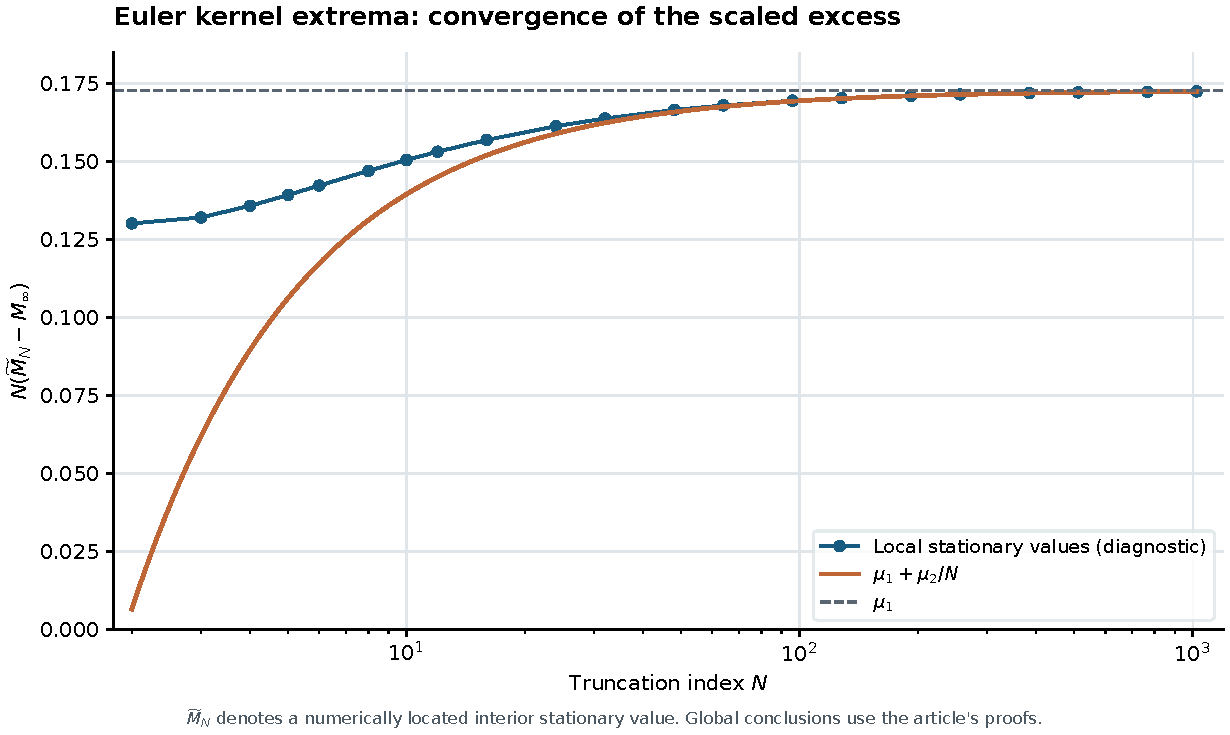
\includegraphics[width=.94\textwidth]{figures/kernel_asymptotics.pdf}
 \caption{Approach to the first two correction terms. The plotted
 $\widetilde M_N$ are values at numerically found interior stationary
 points, with local Hessians checked. They are diagnostics, not
 additional global certificates at the plotted finite indices.
 The global large-$N$ assertion and the coefficients are proved in
 Theorem~\ref{ker:thm:analytic}.}
 \label{ker:fig:asymptotics}
\end{figure}

\section{The optimal order-averaged Euler constant}
\label{ord:sec:main}
The incoming report \cite[Sections 2 and 9]{IncomingBounds} proves
that the optimal order-uniform scaled remainder tends to one and gives
a matching candidate lower asymptotic. Its upper asymptotic remains an
explicit conjecture there. We prove that conjecture, identify the eventual
maximizing boundary, and determine a further asymptotic scale.

Write
\[
 \begin{gathered}
 d_j(a,b)=\sum_{n=0}^j(-1)^n\binom jn
              \frac{H_{2n}^{(b)}}{(2n+1)^a},\qquad
 E_N(a,b)=\sum_{j=0}^{N-1}\frac{d_j(a,b)}{2^{j+1}},\\
 R_N(a,b)=2^N(E_N(a,b)-g_{a,b}).
 \end{gathered}
\]
Let $T_a,U_b$ be independent gamma variables of rate one and shapes
$a,b$, with $T_0=0$. To avoid confusing the logarithmic kernel with the
polylogarithm $F_{a,b}$, put
\begin{equation}\label{ord:eq:psi-J}
 \Psi_N(t)=f_N(e^{-2t}),\qquad J_N(s)=\E\Psi_N(T_s),\qquad J_N(0)=0.
\end{equation}
The existing positive two-measure identity is
\begin{equation}\label{ord:eq:remainder}
 R_N(a,b)=\E\frac{\Psi_N(T_a+U_b)-\Psi_N(T_a)}{1-e^{-U_b}}.
\end{equation}
It holds for $a\ge0,b>0$; in particular it does not require a finite
unweighted signed moment measure. Expanding the denominator into a
positive geometric series and using gamma addition gives, for $b>1$,
\begin{equation}\label{ord:eq:first-gamma}
 0\le R_N(a,b)-\{J_N(a+b)-J_N(a)\}\le\zeta(b)-1.
\end{equation}
For completeness, multiplication of the density of $U_b$ by
$e^{-(r-1)U_b}$ gives $r^{-b}$ times a gamma density of rate $r$.
The term $r=1$ is the displayed difference of $J_N$ values, while each
remaining expectation is between zero and one. Tonelli's theorem
justifies the sum.

We also use the previously proved bound
\begin{equation}\label{ord:eq:inherited-one}
 0<R_N(a,b)<1\qquad(a\ge1,b>0),
\end{equation}
from the manuscript's extended one-sided Euler theorem
\cite[Chapter 5, \texttt{05-real-euler.tex}]{ProveIt}. We identify this
input explicitly: the universal constant greater than one alone would
not replace it in the proof below.

\subsection{Eventual reduction to the outer-order axis}

Define
\begin{equation}\label{ord:eq:axis}
 A_N(b)=R_N(0,b)
 =\frac1{\Gamma(b)}\int_0^\infty t^{b-1}e^{-t}
       k_N(e^{-t})\dd t,
 \qquad
 k_N(v)=\frac{(1+v)(1-v^2)^{N-1}}{1+v^2}.
\end{equation}
All limits of truncation indices in this section are through positive
integers.

\begin{theorem}[Eventual exact axis reduction]\label{ord:thm:axis-reduction}
For all sufficiently large $N$,
\begin{equation}\label{ord:eq:axis-reduction}
 C_N:=\sup_{a,b>0}R_N(a,b)=\max_{b>0}A_N(b)>1.
\end{equation}
The supremum over positive orders is not attained. If $a=0$ is admitted,
every global maximizer is on that axis. Moreover, $C_{N+1}<C_N$ for
all sufficiently large $N$.
\end{theorem}

\begin{proof}
Put $L=\log N$. We separate $b\ge3L/2$ from $b\le3L/2$, always
assuming $N$ large enough for the indicated intervals to be nonempty.

\emph{Comparison above the cutoff.}
The function $f_N$ is decreasing and convex on $[0,1]$, and
$0\le-f_N'(x)\le N+1$. Thus, for $0\le r,v\le1$,
\[
 f_N(rv^2)-f_N(v^2)\le(N+1)(1-r)v^2.
\]
Subtract the axis integrand from \eqref{ord:eq:remainder} and set
$r=e^{-2T_a}$, $v=e^{-U_b}$. Independence gives the useful uniform
comparison
\begin{equation}\label{ord:eq:axis-comparison}
 \begin{split}
 R_N(a,b)-A_N(b)\le{}&
 (N+1)(1-3^{-a})\{\zeta(b)-1-2^{-b}\}\\
 &-J_N(a)\zeta(b),\qquad b>1.
 \end{split}
\end{equation}
Indeed $\E(1-r)=1-3^{-a}$,
$\E[v^2/(1-v)]=\zeta(b)-1-2^{-b}$, and
$\E[1/(1-v)]=\zeta(b)$.

For $0<a\le1$ there is an elementary lower bound
\begin{equation}\label{ord:eq:J-lower}
 J_N(a)\ge\frac{ae^{-2}}{L+4}N^{-1/2}.
\end{equation}
To prove it, restrict the defining integral to
$t\in[L/2+1,L/2+2]$. Bernoulli's inequality gives
\[
 \Psi_N(t)\ge1-(N+1)e^{-2t}\ge1-2e^{-2}>\frac12.
\]
Log convexity of the gamma function gives $\Gamma(a+1)\le1$ for
$0\le a\le1$, and hence $1/\Gamma(a)\ge a$. Also
$t^{a-1}\ge1/t$ on the interval in question, and
$e^{-t}\ge e^{-2}N^{-1/2}$. Its length is one, proving
\eqref{ord:eq:J-lower}.

For $b\ge2$, integral comparison gives
\[
 \zeta(b)-1-2^{-b}
 \le3^{-b}\left(1+\frac3{b-1}\right)\le4\,3^{-b}.
\]
Consequently the positive term in \eqref{ord:eq:axis-comparison}, for
$0<a\le1$ and $b\ge3L/2$, is at most
\[
 8a\log3\,N^{1-(3/2)\log3}.
\]
Its ratio to the right side of \eqref{ord:eq:J-lower} is bounded by
\[
 8e^2\log3\,(L+4)
       e^{-(3/2)(\log3-1)L}\longrightarrow0.
\]
We have therefore proved, uniformly on this parameter region,
\begin{equation}\label{ord:eq:strict-axis-gap}
 R_N(a,b)\le A_N(b)-\frac{ae^{-2}}{2(L+4)}N^{-1/2}
 \qquad(0<a\le1,\ b\ge3L/2)
\end{equation}
for all sufficiently large $N$.

\emph{Exclusion below the cutoff.}
Monotonicity of $J_N$ in its gamma shape and
\eqref{ord:eq:first-gamma} give
\begin{equation}\label{ord:eq:small-b-upper}
 R_N(a,b)\le J_N(b+1)+\zeta(b)-1
       \qquad(0\le a\le1,\ b>1).
\end{equation}
Since $\Psi_N(L/2)=f_N(1/N)\le e^{-1}$,
\begin{equation}\label{ord:eq:deficit-cdf}
 1-J_N(s)\ge(1-e^{-1})
          \Pr\{T_s\le L/2\}.
\end{equation}
For every fixed $D>1/2$ there is $c_D>0$ such that
\begin{equation}\label{ord:eq:gamma-lower-tail}
 \Pr\{T_{DL+1}\le L/2\}
 \ge c_D L^{-1/2}e^{-I(D)L},\qquad
 I(D)=\frac12-D+D\log(2D),
\end{equation}
for all sufficiently large $L$. This lower bound follows directly by
integrating the gamma density over $[L/2-1,L/2]$:
\[
 \Pr\{T_{DL+1}\le L/2\}
 \ge\frac{(L/2-1)^{DL}e^{-L/2}}{\Gamma(DL+1)}.
\]
Stirling's formula \cite[Section 5.11]{DLMF} supplies
\eqref{ord:eq:gamma-lower-tail}; no
large-deviation equivalence is needed.

On $4\le b\le L/2$, gamma stochastic ordering and the central limit
theorem imply that the lower bound in \eqref{ord:eq:deficit-cdf}
eventually exceeds $1/5$ uniformly, since at the worst endpoint
$\Pr\{T_{L/2+1}\le L/2\}\to1/2$. The central limit theorem here follows
from
\[
 \E e^{it(T_s-s)/\sqrt s}
 =e^{-it\sqrt s}(1-it/\sqrt s)^{-s}\longrightarrow e^{-t^2/2}.
\]
On the other hand $\zeta(b)-1\le\zeta(4)-1\le5/48<1/5$.
On $L/2\le b\le L$, apply \eqref{ord:eq:gamma-lower-tail} with $D=1$.
The deficit is bounded below by a positive constant times
\[
 L^{-1/2}N^{-(\log2-1/2)},
\]
whereas $\zeta(b)-1\le2N^{-(\log2)/2}$. The former dominates because
$\log2-1/2<(\log2)/2$.
On $L\le b\le3L/2$, take $D=3/2$. The corresponding deficit is at least
a positive constant times
\[
 L^{-1/2}N^{-((3/2)\log3-1)},
\]
whereas $\zeta(b)-1\le2N^{-\log2}$. Again the deficit dominates:
$(3/2)\log3-1<\log2$. The last inequality is equivalent to
$3\sqrt3<2e$; for example $e>8/3$ and $3\sqrt3<16/3$ prove it.
Thus \eqref{ord:eq:small-b-upper} is strictly below one throughout
$4\le b\le3L/2$ for large $N$.

The bounded rectangle $0\le a\le1$, $0<b\le4$ is also uniform.
Couple $T_a\le T_1$ and $U_b\le U_4$. The derivative satisfies
$0\le\Psi_N'\le4$, and its supremum on every bounded interval tends
to zero. Indeed, with $v=e^{-2t}$, its two positive terms are bounded
by $2Nv(1-v)^{N-1}\le2$ and $2v/(1+v)^2\le1/2$.
The actual terms contain $(1-v)^{N-1}$ and $(1-v)^N$, respectively,
which give uniform decay on every fixed bounded $t$-interval.
Since $u/(1-e^{-u})\le1+u$, we obtain
\[
 R_N(a,b)\le\E\left[(1+U_4)
          \sup_{0\le t\le T_1+U_4}\Psi_N'(t)\right].
\]
The integrand tends to zero and is bounded by $4(1+U_4)$.
Dominated convergence therefore proves uniform convergence to zero on
the bounded rectangle and completes the exclusion below $3L/2$.

Finally, \eqref{ord:eq:inherited-one} excludes $a\ge1$. The function
$A_N$ is continuous, tends to zero as $b\downarrow0$ for $N\ge2$, and
tends to one as $b\to\infty$. The elementary expansion established
below shows that $A_N(b)>1$ for all sufficiently large $b$ at each fixed
$N$. Its maximum is therefore attained and exceeds one. Every positive
outer order is strictly inferior either to one or to its corresponding
axis value, while continuity as $a\downarrow0$ approaches each axis
value. Finally, $A_{N+1}(b)<A_N(b)$ at every $b>0$ by its positive
integral. If $b'$ maximizes $A_{N+1}$ and both indices are in the proved
range, then
\[
 C_{N+1}=A_{N+1}(b')<A_N(b')\le C_N.
\]
This proves eventual strict monotonicity as well.
\end{proof}

\subsection{Resolution of the asymptotic-constant conjecture}

Set
\begin{equation}\label{ord:eq:constants}
 \begin{gathered}
 h=\log(3/2),\qquad \alpha=h^{-1},\qquad
 p=\frac{\log2}{h},\qquad q=\frac{\log3}{\log2},\\
 d_0=\alpha\log q,\qquad
 \widehat b_N=\alpha\log N+d_0=\frac{\log(Nq)}h,\qquad
 c=(1-q^{-1})q^{-p}.
 \end{gathered}
\end{equation}

\begin{lemma}[Axis sign changes and a Taylor enclosure]\label{ord:lem:axis}
For $N\ge2$, $k_N(v)-1$ has exactly one zero in $(0,1)$, with positive
sign before it and negative sign after it. Consequently, if
$A_N(b_0)<1$, then $A_N(b)<1$ for $0<b<b_0$.
For every $N\ge1$ and $b>0$,
\begin{equation}\label{ord:eq:axis-taylor}
 \begin{split}
 A_N(b)&=1+2^{-b}-N3^{-b}-N4^{-b}+\eps_N(b),\\
 0&\le\eps_N(b)\le\frac{N^2-N+2}{2}(5^{-b}+6^{-b}).
 \end{split}
\end{equation}
\end{lemma}
\begin{proof}
The numerator determining the sign of the logarithmic derivative of
$k_N$ on $(0,1)$ is
\[
 P_N(v)=1-(2N+1)v+v^2+(3-2N)v^3.
\]
For $N\ge2$, its derivative is strictly negative on $[0,1]$.
Since $P_N(0)>0>P_N(1)$, the function $k_N$ first increases and then
decreases. Its endpoint values are one and zero, proving the claimed
single crossing.
In the variable $t=-\log v$, the signed function $k_N(e^{-t})-1$ is
negative before a unique $t_0>0$ and positive after it. If $b<b_0$,
multiplication by $t^{b-b_0}$ changes its integral by at most multiplication
by $t_0^{b-b_0}$: the factor is larger on the negative part and smaller
on the positive part. This proves the implication for $A_N$ after
normalizing by the positive gamma factors.

For the enclosure put $G_N(x)=(1-x)^{N-1}/(1+x)$. Its second derivative
is nonnegative and bounded by $N^2-N+2$ on $[0,1]$. For $N\ge3$,
\[
 G_N''(x)=
 \frac{(N-1)(N-2)(1-x)^{N-3}}{1+x}
 +\frac{2(N-1)(1-x)^{N-2}}{(1+x)^2}
 +\frac{2(1-x)^{N-1}}{(1+x)^3};
\]
$N=1,2$ are checked directly. Since $G_N(0)=1$ and $G_N'(0)=-N$,
Taylor's integral remainder gives
\[
 0\le G_N(x)-1+Nx\le\frac{N^2-N+2}{2}x^2.
\]
Multiply by $1+v$, substitute $x=v^2$, and use
$\E e^{-jU_b}=(j+1)^{-b}$.
\end{proof}

\begin{theorem}[Sharp late Euler constant and unique axis maximizer]
\label{ord:thm:leading}
The conjecture of \cite[Section 9]{IncomingBounds} holds:
\begin{equation}\label{ord:eq:sharp-asymptotic}
 C_N-1\sim cN^{-p}.
\end{equation}
For all sufficiently large $N$, $A_N$ has a unique global maximizer
$b_N$, and
\begin{equation}\label{ord:eq:axis-location}
 b_N-\widehat b_N\longrightarrow0.
\end{equation}
\end{theorem}
\begin{proof}
The elementary function $2^{-b}-N3^{-b}$ has its unique maximum at
$b=\widehat b_N$, where its value is $cN^{-p}$. At that point the
remaining terms in \eqref{ord:eq:axis-taylor} are $o(N^{-p})$:
\[
 N4^{-\widehat b_N}=O(N^{1-2p}),\qquad
 N^2 5^{-\widehat b_N}=O(N^{2-\log5/h}).
\]
Here $p>1$, and $\log5/h>p+2$ is equivalent to $5>9/2$. This proves
the required lower asymptotic.

For the upper bound, take $L=\log N$ and first evaluate at $b=2L$.
Divide \eqref{ord:eq:axis-taylor}, minus one, by $N3^{-b}$. The positive
leading ratio is $N^{2h-1}\to0$, and the remainder ratio is
$O(N^{1-2\log(5/3)})\to0$. Thus $A_N(2L)<1$ eventually. The single
crossing from Lemma~\ref{ord:lem:axis} excludes all $b\le2L$.
For $b\ge2L$, the same enclosure gives
\begin{equation}\label{ord:eq:axis-upper-model}
 A_N(b)-1\le2^{-b}-(1-\delta_N)N3^{-b},\qquad
 \delta_N=2N(3/5)^{2L}\longrightarrow0.
\end{equation}
The unrestricted maximum of its right side is
$c\{(1-\delta_N)N\}^{-p}$. Theorem~\ref{ord:thm:axis-reduction} now
proves \eqref{ord:eq:sharp-asymptotic}.

This argument also localizes all near maximizers at the scale of the
excess. Write $b=\widehat b_N+d$. If
$A_N(b)-1\ge(c-o(1))N^{-p}$, \eqref{ord:eq:axis-upper-model} first forces
$d$ into a compact interval: its normalized right side tends to zero
as $d\to+\infty$, and is negative for sufficiently negative $d$.
On compact $d$ intervals,
\begin{equation}\label{ord:eq:profile}
 N^p\{A_N(\widehat b_N+d)-1\}
 \longrightarrow q^{-p}\{2^{-d}-q^{-1}3^{-d}\}
\end{equation}
uniformly. The limiting function has its unique maximum at $d=0$,
so all global maximizers satisfy \eqref{ord:eq:axis-location}.

Convergence in \eqref{ord:eq:profile} holds with two derivatives.
Here is a direct justification for differentiating the remainder.
The first derivative of the normalized gamma density inserts
$\log t-\psi(b)$, and the second inserts
$(\log t-\psi(b))^2-\psi_1(b)$. Under a gamma law of rate $m$,
\[
 \E(\log T-\psi(b))^2=(\log m)^2+\psi_1(b).
\]
Therefore, by the positive bound for the Taylor remainder, its first
two derivative errors are bounded by constants times
$N^2(5^{-b}+6^{-b})$, uniformly for large $b$. The explicit term
$N4^{-b}$ has the same negligible derivative property.
At $d=0$, the limiting second derivative is
\begin{equation}\label{ord:eq:Q-curvature}
 -Q,\qquad Q=(\log2)h q^{-p}>0.
\end{equation}
Every global maximizer eventually lies in a fixed neighborhood where the
second derivative is strictly negative. Strict concavity there proves
uniqueness.
\end{proof}

\subsection{A second asymptotic scale from the gamma threshold}

The next Taylor moment in \eqref{ord:eq:axis-taylor} is a useful bound,
but it is not the next asymptotic term at the moving maximizing order.
The correction comes from the layer $t\simeq(\log N)/2$.
Define
\begin{equation}\label{ord:eq:next-constants}
 \begin{gathered}
 \kappa=\frac12-\alpha+\alpha\log(2\alpha),\qquad
 s=\frac12-\alpha,\\
 D=\sqrt{\frac{\alpha}{2\pi}}(2\alpha)^{-d_0}\Gamma(s).
 \end{gathered}
\end{equation}
The constants satisfy $3/2<\alpha<5/2$, so $-2<s<-1$ and $D>0$.
Elementary logarithm bounds give $p<\kappa<2p-1$. Their approximate
values, used only for orientation, are
\[
 \begin{aligned}
 p&=1.70951129135\ldots,&\qquad
 \kappa&=1.96959041447\ldots,\\
 c&=0.16794779654\ldots,&
 D&=1.56777020071\ldots.
 \end{aligned}
\]

\begin{lemma}[Threshold-layer expansion]\label{ord:lem:threshold}
Fix any $\alpha\in(3/2,5/2)$, independently of its particular value in
\eqref{ord:eq:constants}, and let $b=\alpha L+d$, $L=\log N$, with $d$
in a compact interval. For the exact remainder in
\eqref{ord:eq:axis-taylor},
\begin{equation}\label{ord:eq:threshold-expansion}
 \begin{split}
 \eps_N(\alpha L+d)
 ={}&\sqrt{\frac\alpha{2\pi}}(2\alpha)^{-d}
      N^{-I(\alpha)}L^{-1/2}\\
 &\mathrel{}\times\left\{\Gamma(s)+\frac{B_1(d)}L+O(L^{-2})\right\},
 \qquad s=\frac12-\alpha,
 \end{split}
\end{equation}
where $I$ is as in \eqref{ord:eq:gamma-lower-tail}, and
\begin{equation}\label{ord:eq:B1}
 \begin{split}
 B_1(d)={}&\left\{\frac{d-d^2}{2\alpha}-\frac1{12\alpha}\right\}\Gamma(s)
 -(d-1)\Gamma'(s)-\frac\alpha2\Gamma''(s).
 \end{split}
\end{equation}
The expansion is uniform with any fixed finite number of $d$ derivatives.
It extends to every finite order in $L^{-1}$.
\end{lemma}
\begin{proof}
Set
\[
 G_N(x)=\frac{(1-x)^{N-1}}{1+x},\qquad
 r_N(z)=G_N(z/N)-1+z\quad(0\le z\le N).
\]
Convexity and Lemma~\ref{ord:lem:axis} imply the uniform bound
\begin{equation}\label{ord:eq:remainder-domination}
 0\le r_N(z)\le\min(z,z^2)\qquad(N\ge2).
\end{equation}
Moreover $r_N(z)\to r(z):=e^{-z}-1+z$ on compact $z$ intervals.
The substitution $z=Ne^{-2t}$ in the exact gamma integral gives
\begin{equation}\label{ord:eq:exact-threshold}
 \begin{split}
 \eps_N(b)={}&\frac{N^{-1/2}(L/2)^{b-1}}{2\Gamma(b)}
 \int_0^N z^{-1/2}
       \left(1-\frac{\log z}L\right)^{b-1}\\
 &\hspace{28mm}\mathrel{}\times
       \left(1+\sqrt{\frac zN}\right)r_N(z)\dd z.
 \end{split}
\end{equation}
The factor involving $L$ tends to $z^{-\alpha}$. The limiting integral is
\begin{equation}\label{ord:eq:gamma-mellin}
 \int_0^\infty z^{-\alpha-1/2}(e^{-z}-1+z)\dd z
       =\Gamma(1/2-\alpha).
\end{equation}
Two integrations by parts prove this identity; both endpoint terms
vanish because $3/2<\alpha<5/2$. In particular the individual divergent
integrals of the three summands are never separated.

To justify convergence, choose
$0<\eta<\min(5/2-\alpha,\alpha-3/2)$. For large $L$, the factor in
\eqref{ord:eq:exact-threshold} is bounded by $z^{-\alpha-\eta}$ on
$0<z<1$, and by $z^{-\alpha+\eta}$ on $1<z<N$.
Together with \eqref{ord:eq:remainder-domination} and
$1+\sqrt{z/N}\le2$, these are integrable majorants at both endpoints.
This proves the leading integral limit.

For the expansion put $w=\log z$ and split at $|w|\le L^\theta$, where
$\theta>0$ is sufficiently small for the desired finite expansion order.
The tails have integrable exponential envelopes in $|w|$, so their
integrals are smaller than every inverse power of $L$. On the central
interval,
\begin{equation}\label{ord:eq:log-expansion}
 (b-1)\log(1-w/L)+\alpha w
 =-\frac{(d-1)w+\alpha w^2/2}{L}
   +O\!\left(\frac{|w|^2+|w|^3}{L^2}\right).
\end{equation}
Removal of $\sqrt{z/N}$ and replacement of $r_N$ by $r$ contribute
errors smaller than every inverse power of $L$. For the latter,
the linear term cancels exactly; on the central interval expansion of
$\log G_N(z/N)$ gives
\[
 |G_N(z/N)-e^{-z}|\le C N^{-1}z^2e^{-z}
\]
for large $N$. The logarithmic moments from
\eqref{ord:eq:log-expansion} are the derivatives of the convergent
Mellin integral \eqref{ord:eq:gamma-mellin}. Taylor remainders are
controlled by the same exponential envelopes with additional polynomial
factors in $|w|$.

Stirling's expansion supplies
\begin{equation}\label{ord:eq:stirling-threshold}
 \begin{split}
 \frac{N^{-1/2}(L/2)^{b-1}}{2\Gamma(b)}
 ={}&\sqrt{\frac\alpha{2\pi}}(2\alpha)^{-d}
       N^{-I(\alpha)}L^{-1/2}\\
 &\mathrel{}\times\left[1+\frac1L
       \left\{\frac{d-d^2}{2\alpha}-\frac1{12\alpha}\right\}
         +O(L^{-2})\right].
 \end{split}
\end{equation}
Combining \eqref{ord:eq:log-expansion}--\eqref{ord:eq:stirling-threshold}
proves \eqref{ord:eq:B1}. The argument works at every fixed finite
order. Differentiation in $d$ inserts powers of $\log(1-w/L)$ in the
integral and logarithmic derivatives of the gamma prefactor. On $w<0$,
$\log(1+|w|/L)\le |w|/L$. On $0<w<L$, each fixed power of
$|\log(1-w/L)|$ can be absorbed by decreasing the positive exponent
$b-1$ by $\eta L$: for $0<u<1$,
\[
 u^{\eta L}|\log u|^j\le\left(\frac{j}{e\eta L}\right)^j
 \quad(j\ge1).
\]
Choosing the initial $\eta$ with a further factor of two of room leaves
the same integrable exponential tails. The gamma-prefactor derivatives
remain bounded after normalization, by Stirling's differentiated
expansion. These estimates apply in particular through two derivatives,
and prove all the asserted uniform derivatives.
\end{proof}

\begin{theorem}[Second scale and displacement of the maximizing order]
\label{ord:thm:second}
With the constants in \eqref{ord:eq:constants},
\eqref{ord:eq:Q-curvature}, and \eqref{ord:eq:next-constants},
\begin{equation}\label{ord:eq:second-asymptotic}
 C_N=1+cN^{-p}
       +DN^{-\kappa}(\log N)^{-1/2}
            \{1+O((\log N)^{-1})\},
\end{equation}
and the unique axis maximizing order satisfies
\begin{equation}\label{ord:eq:displacement}
 b_N=\widehat b_N-\frac{D\log(2\alpha)}Q
            N^{-(\kappa-p)}(\log N)^{-1/2}
            \{1+O((\log N)^{-1})\}.
\end{equation}
More precisely, the braces in \eqref{ord:eq:second-asymptotic} begin
$1+B/\log N+O((\log N)^{-2})$, where
\begin{equation}\label{ord:eq:relative-B}
 B=\frac{d_0-d_0^2}{2\alpha}-\frac1{12\alpha}
       -(d_0-1)\psi(s)
       -\frac\alpha2\{\psi_1(s)+\psi(s)^2\}.
\end{equation}
An expansion through every finite inverse power of $\log N$ at this
second scale is obtained by the same Mellin-moment procedure.
\end{theorem}
\begin{proof}
At $b=\widehat b_N$, Lemma~\ref{ord:lem:threshold} applies with $d=d_0$.
The explicit term $N4^{-b}$ in \eqref{ord:eq:axis-taylor} is
$O(N^{-(2p-1)})$, smaller than $N^{-\kappa}(\log N)^{-m}$ for every
fixed $m$. This proves the stated expansion first at $\widehat b_N$.

For the optimizer, Theorem~\ref{ord:thm:leading} already gives
$b_N-\widehat b_N=o(1)$ and uniform negative curvature of order $N^{-p}$.
At $\widehat b_N$ the derivative of the elementary leading pair vanishes.
The derivative version of Lemma~\ref{ord:lem:threshold} shows that the
remaining derivative is
\[
 -D\log(2\alpha)N^{-\kappa}L^{-1/2}\{1+O(L^{-1})\}.
\]
The leading second derivative is $-QN^{-p}$. The mean-value theorem
first gives $b_N-\widehat b_N=O(N^{-(\kappa-p)}L^{-1/2})$, and then
substitution back into that derivative equation gives
\eqref{ord:eq:displacement}. The change in the maximum's value is
$O(N^{-(2\kappa-p)}L^{-1})$, smaller than every
$N^{-\kappa}L^{-m}$ at fixed $m$. The whole second-scale inverse-log
expansion therefore transfers unchanged from $\widehat b_N$ to the
maximum. Division of \eqref{ord:eq:B1} by $\Gamma(s)$ gives
\eqref{ord:eq:relative-B}.
\end{proof}

\begin{remark}[A particularly late asymptotic regime]\label{ord:rem:late}
The inequalities $3/2<\alpha<5/2$ are essential. Here
$5/2-\alpha=0.0336965\ldots$ is small, and the lower endpoint of the
Mellin integral decays slowly. The coefficient in
\eqref{ord:eq:relative-B} is correspondingly large in magnitude.
The formulas are proved asymptotics as $N\to\infty$, without a claim
that the second term is accurate at ordinary numerical truncation
indices. In particular replacing it by the next Taylor moment
$N^2 5^{-\widehat b_N}/2$ would be incorrect: its exponent
$\log5/h-2$ is strictly smaller than $\kappa$, and its ratio to the
true second-scale correction grows without bound.
\end{remark}

\subsection{What sufficiently accurate near maximizers must do}

\begin{lemma}[A uniform small-outer-order tail]\label{ord:lem:small-shape}
Uniformly for $0<a\le1$,
\begin{equation}\label{ord:eq:small-shape}
 J_N(a)=\frac{\sqrt\pi}{2^a\Gamma(a)}
              N^{-1/2}(\log N)^{a-1}\{1+o(1)\}.
\end{equation}
In particular, if $a\to0$ and $a\log\log N\to0$, then
$J_N(a)\sim\sqrt\pi\,aN^{-1/2}/\log N$.
\end{lemma}
\begin{proof}
With $L=\log N$ and $z=Ne^{-2t}$,
\[
 J_N(a)=\frac{N^{-1/2}(L/2)^{a-1}}{2\Gamma(a)}
 \int_0^N z^{-1/2}
   \left(1-\frac{\log z}L\right)^{a-1}f_N(z/N)\dd z.
\]
On $0<z\le\sqrt N$, the factor raised to $a-1$ is bounded by one
for $z<1$ and by two for $z\ge1$. Also $f_N(z/N)\le e^{-z}$.
The factor tends to one uniformly in $a\in(0,1]$ at each fixed $z$,
so dominated convergence gives $\Gamma(1/2)$ from this part, uniformly
in $a$.
The remaining part corresponds to $t<L/4$. For $0<t<1$, put
$\rho=1-e^{-2}<1$ and use
$(1-e^{-2t})^N\le2t\rho^{N-1}$. For $1<t<L/4$ use
$\Psi_N(t)\le e^{-\sqrt N}$. Since $1/\Gamma(a)=O(a)$ uniformly on
$(0,1]$, this part of $J_N(a)$ is
$O(a\rho^{N-1}+ae^{-\sqrt N})$, negligible relative to the proposed
main term uniformly in $a$. This proves \eqref{ord:eq:small-shape}.
Finally $\Gamma(a)^{-1}\sim a$ and
$(L/2)^a\to1$ under the stated hypotheses.
\end{proof}

\begin{proposition}[Two-scale local profile in the order plane]
\label{ord:prop:order-profile}
Suppose $a_N\ge0$, $b_N>0$, and
\[
 \frac{a_N}{(\log N)N^{-(p-1/2)}}\longrightarrow u\ge0,
 \qquad b_N-\widehat b_N\longrightarrow d\in\R.
\]
Then
\begin{equation}\label{ord:eq:order-profile}
 N^p\{R_N(a_N,b_N)-1\}
 \longrightarrow
 q^{-p}\{2^{-d}-q^{-1}3^{-d}\}-\sqrt\pi\,u.
\end{equation}
\end{proposition}
\begin{proof}
The exact difference used in \eqref{ord:eq:axis-comparison} has the form
\[
 R_N(a,b)-A_N(b)=-J_N(a)\zeta(b)+\Delta_N(a,b),
\]
where
\[
 0\le\Delta_N(a,b)\le
 (N+1)(1-3^{-a})\{\zeta(b)-1-2^{-b}\}.
\]
At $b=\widehat b_N+O(1)$ the latter bound is $O(aN^{-p})$.
Under the hypothesis $a_N\to0$, so this is $o(N^{-p})$.
Lemma~\ref{ord:lem:small-shape} gives
$N^pJ_N(a_N)\to\sqrt\pi\,u$; the same conclusion is immediate at
$a_N=0$. Also $\zeta(b_N)\to1$. Combine this with
\eqref{ord:eq:profile}.
\end{proof}



\begin{corollary}[Quantitative approach to the maximizing boundary]
\label{ord:cor:near-maximizers}
Suppose $a_N,b_N>0$. The condition
\[
 C_N-R_N(a_N,b_N)=o(N^{-p})
\]
is equivalent to
\begin{equation}\label{ord:eq:near-maximizers}
 a_N=o\!\left(N^{-(p-1/2)}\log N\right),\qquad
 b_N-\widehat b_N\longrightarrow0.
\end{equation}
\end{corollary}
\begin{proof}
The hypothesis and Theorem~\ref{ord:thm:leading} imply
$R_N(a_N,b_N)>1$ eventually. The exclusion argument in
Theorem~\ref{ord:thm:axis-reduction} forces $0<a_N<1$ and
$b_N>3\log N/2$. Since $A_N(b_N)\le C_N$,
\eqref{ord:eq:strict-axis-gap} gives the first conclusion.
It also shows $A_N(b_N)-1\ge(c-o(1))N^{-p}$, so the localization proof
in Theorem~\ref{ord:thm:leading} gives the second.
Conversely, \eqref{ord:eq:near-maximizers} gives $u=d=0$ in
Proposition~\ref{ord:prop:order-profile}; its limit is $c$, which is also
the limit of $N^p(C_N-1)$.
\end{proof}

The accuracy $o(N^{-p})=o(C_N-1)$ matters. An error merely $o(1)$
allows the broad moving-order phase region already present in the
incoming report and need not force the outer order to zero. The results
above prove eventual strict monotonicity through the exact axis reduction,
while monotonicity for the entire sequence remains open. A theorem covering
all finite truncation indices and an effective threshold for the eventual
statements remain concrete further problems.

\begin{figure}[htbp]
 \centering
 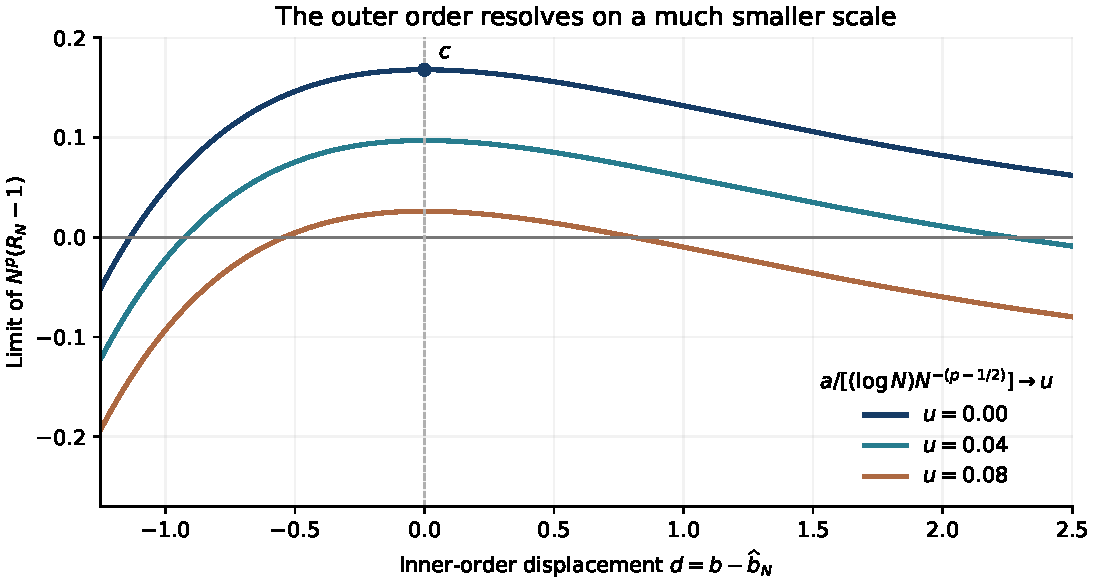
\includegraphics[width=.93\textwidth]{figures/order_plane_profile.pdf}
 \caption{The exact limiting function in
 Proposition~\ref{ord:prop:order-profile}, at three values of the scaled
 outer order $u$. The maximum $c$ occurs at $u=d=0$. These curves depict
 the proved limit; they are not finite-$N$ approximation error claims.}
 \label{ord:fig:profile}
\end{figure}

\section{Polynomial Appell mesh and uniform Lerch zero thresholds}
\label{mesh:sec:main}

The incoming uniform-continuation article asks whether the roots of the
reciprocal-gamma Appell polynomials admit a polynomial lower separation
bound. Its estimate $(3n)^{-(n-2)}$ gives an effective zero theorem, but
only a logarithmic growing-index range. We prove
\begin{equation}\label{mesh:eq:main-mesh}
 \boxed{\mesh(Q_n)\geq\frac1{10n^2}\qquad(n\geq2).}
\end{equation}
A second improvement replaces a worst-distance estimate by a harmonic
sum over the entire root configuration. Together these give a sufficient
Lerch saturation threshold of order $n^4\log^2 n$, and a relative
location error independent of $n$. The constants below are explicit
and deliberately conservative; no sharp mesh asymptotic is asserted.

\subsection{Definitions and the strengthened zero theorem}

Define the monic Appell polynomials by
\begin{equation}\label{mesh:eq:Q}
 \frac{e^{xt}}{\Gamma(1+t)}
   =\sum_{n\geq0}Q_n(x)\frac{t^n}{n!},
 \qquad W_\rho(t)=\frac1{1-\rho e^{-t}}\quad(0\leq\rho\leq1).
\end{equation}
For $n\geq0$, $k\geq1$ and $a>0$, put
\begin{equation}\label{mesh:eq:family}
 F_{n,k}^\rho(a)=\int_0^\infty
      t^k e^{-at}W_\rho(t)Q_n(\log t)\dd t.
\end{equation}
This is the manuscript's signed derivative family:
\[
 F_{n,k}^\rho=(-1)^{n+k}D_{n,k}^\rho,
 \qquad
 D_{n,k}^\rho(a)=
 \begin{cases}
  \partial_a^k\displaystyle\sum_{m\geq0}
       \dfrac{\rho^m\log^n(a+m)}{a+m},&0\leq\rho<1,\\[2mm]
  \gamma_n^{(k)}(a),&\rho=1.
 \end{cases}
\]
The endpoint $\rho=1$ unifies the derivatives, not the generally
divergent undifferentiated Lerch series. The Mellin derivation of
\eqref{mesh:eq:family} is already established in the manuscript.
We recall below the positive-transform zero bound needed to make
our localization complete.

Write the roots decreasingly as $x_{n,1}>\cdots>x_{n,n}$, set
$c_{n,j}=e^{-x_{n,j}}$, and let $H_r=\sum_{h=1}^r h^{-1}$.

\begin{theorem}[Polynomial threshold and simultaneous location]
\label{mesh:thm:saturation}
For $n\geq2$, define the explicit integer
\begin{equation}\label{mesh:eq:threshold}
 K_n=\left\lceil\bigl(16+240n^2H_{n-1}\bigr)^2\right\rceil.
\end{equation}
For every integer $k\geq K_n$ and every $\rho\in[0,1]$,
$F_{n,k}^\rho$ has exactly $n$ positive zeros, all simple.
Numbering them increasingly as $a_{n,j,k}^\rho$, one has
\begin{equation}\label{mesh:eq:location}
 \boxed{\left|\log\frac{a_{n,j,k}^\rho}{k c_{n,j}}\right|
          <\frac8{\sqrt{k}},\qquad 1\leq j\leq n.}
\end{equation}
All assertions hold simultaneously over the entire deformation interval
and over the smallest and largest zero; no compact restriction on the
slopes $c_{n,j}$ is needed.
\end{theorem}

The proof is divided into an algebraic separation theorem and a
scale-free analytic sign-transfer theorem.

\subsection{Two distinct monotonicity statements for differential factors}

For a real-rooted polynomial, its mesh is the minimum spacing of
consecutive roots counted with multiplicity. Thus a multiple root gives
mesh zero. In this subsection $\partial$ means differentiation in $x$.

\begin{lemma}[Coordinatewise motion of ordered roots]
\label{mesh:lem:motion}
For a fixed real-rooted polynomial $p$, every ordered root of
$p+c p'$, counted with multiplicity, is nonincreasing as $c>0$ increases.
Consequently each ordered root of
\[
 P(x)=\prod_{j=1}^m(1+c_j\partial)x^n
\]
is nonincreasing in each positive parameter $c_j$ separately.
\end{lemma}
\begin{proof}
Let the distinct roots of $p$ be $r_i$, with multiplicities $m_i$.
A root of multiplicity $m_i\geq2$ is inherited with multiplicity
$m_i-1$. All other roots solve
\[
 S(x):=\sum_i\frac{m_i}{x-r_i}=-\frac1c.
\]
There is one solution in each interval between consecutive distinct
roots and one to the left of all roots. Since
$S'(x)=-\sum_i m_i/(x-r_i)^2<0$, these solutions are simple, and
\begin{equation}\label{mesh:eq:root-motion}
 \frac{\dd x}{\dd c}
   =-\frac1{c^2\displaystyle\sum_i m_i/(x-r_i)^2}<0.
\end{equation}
The inherited roots remain fixed. No moving root crosses an inherited
one, because it remains in its designated complementary interval.
This proves the first assertion and real-rootedness preservation.
For the second assertion, hold all parameters except $c_j$ fixed and
apply the first to the real-rooted polynomial produced by the other
factors. The factors commute.
\end{proof}

\begin{lemma}[Riesz mesh preservation]\label{mesh:lem:riesz}
For every real-rooted polynomial $p$ and every real $c$,
\begin{equation}\label{mesh:eq:riesz}
 \mesh(p+c p')\geq\mesh(p).
\end{equation}
\end{lemma}
\begin{proof}
This classical theorem is recorded in~\cite[Theorem~1]{BKS2016}.
Here is the relevant argument. If $0<h<\mesh(p)$, then $p(x)$ and
$p(x-h)$ have interlacing roots. The real-rooted-pencil criterion says
that two real-rooted polynomials interlace if and only if every real
linear combination is real-rooted or zero. To recall why, after common
roots are removed, the partial fractions of their quotient have residues
of one sign precisely in the interlacing case. Its imaginary part then
has a fixed nonzero sign in the upper half-plane, so it takes no real
value there. Conversely, if every real pencil member has real roots,
the quotient takes no real value in that half-plane; continuity fixes
the sign of its imaginary part, and approach to each pole forces the
residues to have a common sign. This gives interlacing. Common roots
can be restored, or treated by limits.

The operator $T=1+c\partial$ preserves real-rootedness and commutes
with translation. Apply it to the interlacing pencil. Every real
combination of $Tp(x)$ and $Tp(x-h)$ remains real-rooted or zero,
so the shifted pair interlaces. For a polynomial and its translate by
$h>0$, this is equivalent to mesh at least $h$. Let $h$ increase to
$\mesh(p)$. If the original mesh is zero, the assertion follows
already from real-rootedness preservation.
\end{proof}

Lemma~\ref{mesh:lem:motion} concerns the location of each root, whereas
Lemma~\ref{mesh:lem:riesz} compares a polynomial with its image under
one operator. We do not claim that the mesh of $p+c p'$ is monotone
as a function of $c$; that stronger statement is false in general.

\subsection{A Laguerre comparison with uniform spacing}

The standard Laguerre coefficient formula, differential equation and
three-term recurrence used here are collected in DLMF
\S\S18.5, 18.8 and 18.9~\cite{DLMF}. We supply the bounds explicitly.

\begin{lemma}[An equal-factor reference polynomial]
\label{mesh:lem:laguerre}
For every $n\geq3$, the roots of
\begin{equation}\label{mesh:eq:laguerre-block}
 (1+\partial)^{3n}x^n=n!L_n^{(2n)}(-x)
\end{equation}
are negative and simple. Every adjacent gap exceeds $3$, and every
root has absolute value less than $15n/2$.
\end{lemma}
\begin{proof}
More generally, for $m\geq n$, direct coefficient comparison gives
\[
 (1+\partial)^m x^n=n!L_n^{(m-n)}(-x),\qquad
 L_n^{(\alpha)}(z)=\sum_{r=0}^n
       (-1)^r\binom{n+\alpha}{n-r}\frac{z^r}{r!}.
\]
Repeated real-root preservation removes all initial multiplicities
after $n-1$ nonzero factors. The resulting polynomial has strictly
positive coefficients when $m\geq n$, so all its real roots are
strictly negative. Equivalently the Laguerre roots are positive
and simple.

Write $y=L_n^{(\alpha)}$. Its differential equation is
\[
 xy''+(\alpha+1-x)y'+ny=0.
\]
The substitution $u=x^{(\alpha+1)/2}e^{-x/2}y$ gives
\begin{equation}\label{mesh:eq:laguerre-normal}
 u''+q(x)u=0,\qquad
 q(x)=\frac{2n+\alpha+1}{2x}
       +\frac{1-\alpha^2}{4x^2}-\frac14.
\end{equation}
For $\alpha=2n$, maximizing the quadratic in $1/x$ yields
\begin{equation}\label{mesh:eq:potential-bound}
 q(x)\leq\frac{12n^2+8n+2}{16n^2-4}\leq1\quad(n\geq3).
\end{equation}
Indeed the difference of denominator and numerator is
$4n^2-8n-6=4(n-3)^2+16(n-3)+6>0$.
If $\lambda_i<\lambda_{i+1}$ are consecutive positive Laguerre roots,
then $u$ vanishes at both endpoints of this interval. Integration by
parts and the Dirichlet Wirtinger inequality imply
\[
 \frac{\pi^2}{(\lambda_{i+1}-\lambda_i)^2}
       \int_{\lambda_i}^{\lambda_{i+1}}u^2\dd x
 \leq\int_{\lambda_i}^{\lambda_{i+1}}(u')^2\dd x
 =\int_{\lambda_i}^{\lambda_{i+1}}q u^2\dd x
 \leq\int_{\lambda_i}^{\lambda_{i+1}}u^2\dd x.
\]
Thus every gap is at least $\pi>3$.

For the largest root, the monic Laguerre recurrence identifies the
zeros with the eigenvalues of the symmetric tridiagonal matrix having
\[
 J_{ii}=2i-1+\alpha\quad(1\leq i\leq n),\qquad
 J_{i,i+1}=J_{i+1,i}=\sqrt{i(i+\alpha)}.
\]
At $\alpha=2n$, each diagonal is at most $4n-1$, and each
nonzero off-diagonal is less than $\sqrt3\,n$. The row-sum
bound for eigenvalues therefore gives
\[
 \lambda_n\leq(4+2\sqrt3)n-1<\frac{15n}{2},
\]
where $\sqrt3<7/4$. This proves both estimates.
\end{proof}

\subsection{Selecting a remote block from the gamma product}

\begin{theorem}[Polynomial reciprocal-gamma root separation]
\label{mesh:thm:polynomial}
For every integer $n\geq2$, $Q_n$ has $n$ distinct real roots and
satisfies \eqref{mesh:eq:main-mesh}.
\end{theorem}
\begin{proof}
First take $n\geq3$, and set $M=15n^2$, $m=3n$. Consider the finite
block
\begin{equation}\label{mesh:eq:remote-block}
 B_n(x)=\prod_{j=M}^{M+m-1}(1+\partial/j)x^n.
\end{equation}
Let $r_1<\cdots<r_n<0$ be the roots of the equal-factor polynomial
in \eqref{mesh:eq:laguerre-block}, and $R_1<\cdots<R_n$ those
of $B_n$. Put $c_+=1/M$ and $c_-=1/(M+m-1)$. Every coefficient
of a differential factor in \eqref{mesh:eq:remote-block} lies
between $c_-$ and $c_+$. Lemma~\ref{mesh:lem:motion}, together
with homogeneity of an equal-factor block, gives
\begin{equation}\label{mesh:eq:sandwich}
 c_+r_i\leq R_i\leq c_-r_i\qquad(1\leq i\leq n).
\end{equation}
The inequalities have this orientation because all $r_i$ are negative.
Write $R_i=c_+r_i+\eps_i$. By Lemma~\ref{mesh:lem:laguerre},
\[
 0\leq\eps_i< E,\qquad
 E=\frac{45n^2}{2M^2},
\]
since
\[
 (c_+-c_-)\frac{15n}{2}
 <\frac{m}{M^2}\frac{15n}{2}=E.
\]
The errors lie on the same side of the reference roots, so each gap
loses at most $E$, not $2E$. Consequently
\begin{equation}\label{mesh:eq:block-bound}
 R_{i+1}-R_i>\frac3M-E
 =\frac3{15n^2}-\frac{45n^2}{2(15n^2)^2}
 =\frac1{10n^2}.
\end{equation}

The Weierstrass product for the reciprocal gamma function yields the
finite-product Appell polynomials
\[
 Q_{n,N}(x)=\prod_{j=1}^N(1+\partial/j)(x+\gamma-H_N)^n.
\]
For every $N\geq M+m-1$, start with the block $B_n$, restore the
remaining factors, and translate by $\gamma-H_N$. All factors and
translations commute. Lemma~\ref{mesh:lem:riesz} shows that the
restored factors cannot decrease mesh; translations preserve it.
Thus $\mesh(Q_{n,N})>1/(10n^2)$.
The locally uniform convergence of the Weierstrass product implies
coefficientwise convergence $Q_{n,N}\to Q_n$. Ordered real roots
of monic fixed-degree polynomials vary continuously with the
coefficients, so the non-strict gap bound passes to the limit.
It proves simplicity as well as real-rootedness of $Q_n$.

Finally $Q_2(x)=(x+\gamma)^2-\zeta(2)$ has mesh
$2\sqrt{\zeta(2)}>2>1/40$, which handles the omitted index.
\end{proof}

The choice of a distant block is useful because its coefficients
$1/j$ vary little across $3n$ successive factors. It supplies separated
roots before any potentially troublesome infinite-product limit is
taken. The remaining gamma factors then preserve this separation.

\subsection{A scale-free sign-transfer estimate}

Let $Y_k$ have the gamma density
\begin{equation}\label{mesh:eq:gamma-density}
 \frac{k^{k+1}}{k!}y^k e^{-ky},\qquad y>0.
\end{equation}
Its shape is $k+1$ and rate is $k$.

\begin{lemma}[An exponential log-moment bound]
\label{mesh:lem:gamma-moment}
For positive integers $m,k$ with $k\geq16m^2$,
\begin{equation}\label{mesh:eq:gamma-moment}
 \E\bigl(e^{m|\log Y_k|}-1\bigr)
 \leq\sqrt{2(e^{4m^2/k}-1)}\leq\sqrt{2/3}<1.
\end{equation}
\end{lemma}
\begin{proof}
The square of $e^{m|\log y|}-1$ is either $(y^m-1)^2$ or
$(y^{-m}-1)^2$, hence is at most their sum. Cauchy--Schwarz bounds
the square of the left side of \eqref{mesh:eq:gamma-moment} by
\[
 \E Y_k^{2m}+\E Y_k^{-2m}-2\E Y_k^m-2\E Y_k^{-m}+2.
\]
The integer moments are
\[
 \E Y_k^r=\prod_{j=1}^r(1+j/k),\qquad
 \E Y_k^{-r}=\prod_{j=0}^{r-1}(1-j/k)^{-1}\quad(r\leq k).
\]
Both products are at least one. Since $k\geq4m$, logarithmic
bounds give
\[
 \log\E Y_k^{2m}\leq\frac{m(2m+1)}k\leq\frac{3m^2}k,
 \qquad
 \log\E Y_k^{-2m}\leq\frac2k\sum_{j=0}^{2m-1}j
                    \leq\frac{4m^2}k.
\]
The second estimate uses $-\log(1-u)\leq2u$ for $0\leq u\leq1/2$.
This proves the first claimed inequality. Finally $4m^2/k\leq1/4$
and $e^{1/4}\leq(1-1/4)^{-1}=4/3$ prove the second.
\end{proof}

\begin{proposition}[Root-distance sign transfer]
\label{mesh:prop:sign}
For real $s$ not a root of $Q_n$, set
\begin{equation}\label{mesh:eq:S}
 S_n(s)=\sum_{\ell=1}^n\frac1{|s-x_{n,\ell}|},
 \qquad m=\lceil1+S_n(s)\rceil.
\end{equation}
If $k\geq16m^2$, then simultaneously for $\rho\in[0,1]$,
\begin{equation}\label{mesh:eq:relative-sign}
 \left|
 \frac{(ke^{-s})^{k+1}F_{n,k}^\rho(ke^{-s})}
      {k!W_\rho(e^s)Q_n(s)}-1
 \right|\leq\sqrt{2/3}<1.
\end{equation}
In particular $F_{n,k}^\rho(ke^{-s})$ and $Q_n(s)$ have the same sign.
\end{proposition}
\begin{proof}
A direct substitution in \eqref{mesh:eq:family} gives the exact identity
\begin{equation}\label{mesh:eq:expectation}
 \frac{(ke^{-s})^{k+1}F_{n,k}^\rho(ke^{-s})}
      {k!W_\rho(e^s)Q_n(s)}
 =\E\left[
 \frac{W_\rho(e^sY_k)}{W_\rho(e^s)}
 \frac{Q_n(s+\log Y_k)}{Q_n(s)}\right].
\end{equation}
The logarithmic derivative of the weight satisfies
\[
 \left|\frac{\dd\log W_\rho(x)}{\dd\log x}\right|
 =\frac{x\rho}{e^x-\rho}\leq1.
\]
Indeed $e^x-\rho\geq1+x-\rho\geq\rho x$. This includes both
endpoints of the deformation interval. For
$R=W_\rho(e^{s+u})/W_\rho(e^s)$ one obtains
$R\leq e^{|u|}$ and $|R-1|\leq e^{|u|}-1$.
The product over polynomial roots gives
\[
 \left|\frac{Q_n(s+u)}{Q_n(s)}-1\right|
 \leq\prod_{\ell=1}^n\left(1+\frac{|u|}{|s-x_{n,\ell}|}\right)-1
 \leq e^{S_n(s)|u|}-1.
\]
Combining the two estimates yields
\[
 \left|R\frac{Q_n(s+u)}{Q_n(s)}-1\right|
 \leq e^{(1+S_n(s))|u|}-1\leq e^{m|u|}-1.
\]
Take expectations in \eqref{mesh:eq:expectation} and apply
Lemma~\ref{mesh:lem:gamma-moment}. These estimates also give the
needed absolute integrability. Since the normalized quantity lies
within distance less than one of $1$, it is positive.
\end{proof}

\subsection{Harmonic root distances and completeness of localization}

\begin{lemma}[Positive-transform zero bound]\label{mesh:lem:zeros}
For $n\geq0$, $k\geq1$ and $0\leq\rho\leq1$, the function
$F_{n,k}^\rho$ has at most $n$ positive zeros, counted with multiplicity.
\end{lemma}
\begin{proof}
A real kernel with $N$ sign changes has a Laplace transform with at
most $N$ positive zeros, counted with multiplicity, when its exponentially
weighted polynomial moments converge. One direct proof is induction.
At a sign-change point $t_0$, multiplication of the kernel by $t_0-t$
removes exactly that sign change. Its transform is
\[
 (\partial_a+t_0)F(a)
  =e^{-t_0a}\frac{\dd}{\dd a}\bigl(e^{t_0a}F(a)\bigr).
\]
Any finite collection of zeros of $F$ with total multiplicity $M$
forces at least $M-1$ zeros of the transformed function by Rolle's
theorem with multiplicities. The induction hypothesis gives $M\leq N$.
The fixed-sign case begins the induction, and the same induction
precludes an identically zero transform.

Here $Q_n(\log t)$ has $n$ simple sign changes, whereas
$t^kW_\rho(t)>0$. The bound
$W_\rho(t)\leq W_1(t)\leq1+t^{-1}$ ensures integrability at zero,
and $e^{-at}$ supplies it at infinity, also after any fixed number
of $a$-derivatives. The variation argument therefore applies.
\end{proof}

\begin{theorem}[Saturation from any mesh bound]
\label{mesh:thm:transfer}
Suppose $n\geq2$ and $\delta>0$ is a proved lower bound for
$\mesh(Q_n)$. If
\begin{equation}\label{mesh:eq:generic-threshold}
 \sqrt{k}\geq16+\frac{24H_{n-1}}\delta,
\end{equation}
then the full zero-count and location conclusions of
Theorem~\ref{mesh:thm:saturation} hold.
\end{theorem}
\begin{proof}
Set $\eta=8/\sqrt{k}$. Since $H_{n-1}\geq1$,
\eqref{mesh:eq:generic-threshold} implies $\eta\leq\delta/3$.
At either endpoint $s=x_{n,j}\pm\eta$, the distinguished root is
at distance $\eta$, while every other root obeys
\[
 |s-x_{n,\ell}|\geq|\ell-j|\delta-\eta
      \geq\frac23|\ell-j|\delta.
\]
Consequently
\begin{align}
 S_n(s)&\leq\frac1\eta+
       \frac3{2\delta}\bigl(H_{j-1}+H_{n-j}\bigr)\notag\\
 &\leq\frac{\sqrt{k}}8+\frac{3H_{n-1}}\delta.
 \label{mesh:eq:harmonic-distance}
\end{align}
Thus
\[
 m=\lceil1+S_n(s)\rceil
 \leq2+\frac{\sqrt{k}}8+\frac{3H_{n-1}}\delta
 \leq\frac{\sqrt{k}}4,
\]
where the last inequality is exactly
\eqref{mesh:eq:generic-threshold}. Proposition~\ref{mesh:prop:sign}
transfers the opposite polynomial signs at both endpoints to the
corresponding values of $F_{n,k}^\rho$, uniformly in $\rho$.

The $n$ intervals $[x_{n,j}-\eta,x_{n,j}+\eta]$ are disjoint,
because $2\eta\leq2\delta/3<\delta$. The decreasing coordinate
change $a=ke^{-s}$ gives $n$ disjoint positive intervals, each with
opposite endpoint signs, hence each containing a zero. By
Lemma~\ref{mesh:lem:zeros} these are all the positive zeros;
each interval contains exactly one, and every zero is simple.
The interval endpoints give \eqref{mesh:eq:location}, with a strict
inequality because the transferred endpoint signs are nonzero.
\end{proof}

\begin{proof}[Proof of Theorem~\ref{mesh:thm:saturation}]
Insert the proved value $\delta=1/(10n^2)$ from
Theorem~\ref{mesh:thm:polynomial} into
Theorem~\ref{mesh:thm:transfer}.
\end{proof}

\paragraph{Combining proved mesh bounds at small degrees.}
The incoming bound $\mesh(Q_n)\ge(3n)^{-(n-2)}$
\cite[Section 4]{IncomingUniform} and
Theorem~\ref{mesh:thm:polynomial} may both be retained. Set
\[
 \delta_n^{\mathrm{comb}}
   =\max\{(3n)^{-(n-2)},\,1/(10n^2)\},\qquad
 K_n^{\mathrm{comb}}
   =\left\lceil\left(16+
             \frac{24H_{n-1}}{\delta_n^{\mathrm{comb}}}\right)^2
     \right\rceil.
\]
Theorem~\ref{mesh:thm:transfer} applies with this bound too.
It uses the better old separation estimate at $n=2,3,4$ and the
polynomial estimate thereafter, while keeping the improved
$8/\sqrt{k}$ location error throughout. These remain sufficient
thresholds, not assertions about the first index at which the zero
count is saturated.

\begin{figure}[tbp]
 \centering
 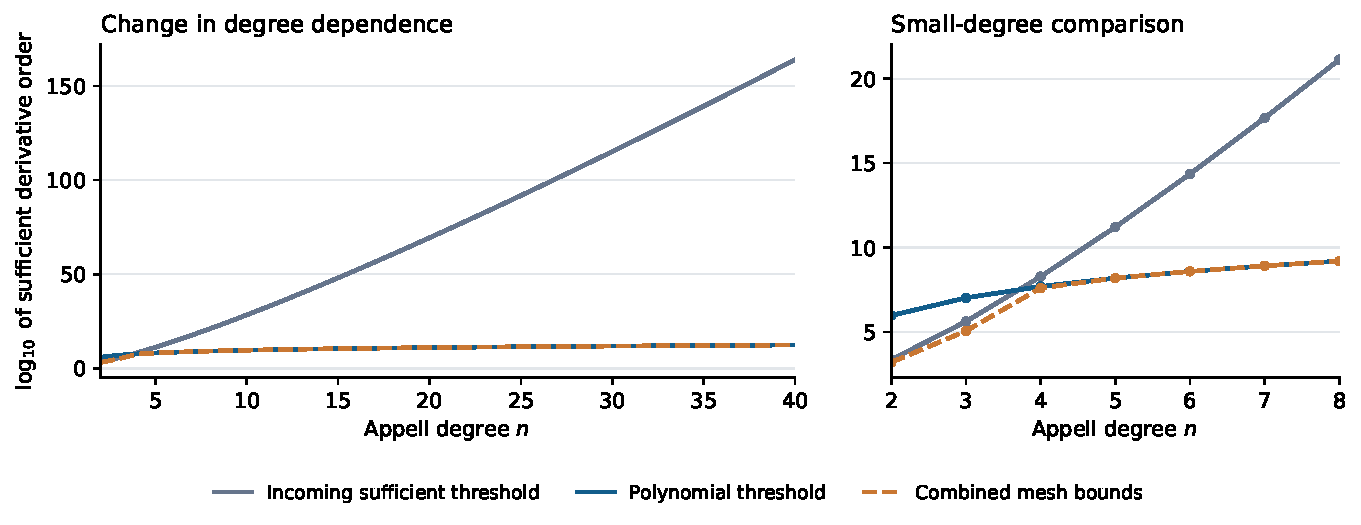
\includegraphics[width=.98\textwidth]{figures/mesh_threshold_comparison.pdf}
 \caption{Comparison of proved sufficient derivative-order thresholds.
 The incoming threshold is $576n^2(3n)^{2n-4}$.
 The polynomial threshold is \eqref{mesh:eq:threshold}, and the
 combined bound uses $\delta_n^{\mathrm{comb}}$ in the improved
 transfer theorem. The ordinate is the base-ten logarithm of each
 integer threshold; no numerical zero search is involved.}
 \label{mesh:fig:thresholds}
\end{figure}

\subsection{A polynomial growing-index regime}

\begin{corollary}[Joint growth of index and derivative order]
\label{mesh:cor:growing}
Fix $0<\alpha<1/\sqrt{60}$. For all sufficiently large integers $k$,
simultaneously for
\begin{equation}\label{mesh:eq:growing-range}
 2\leq n\leq\alpha\frac{k^{1/4}}{\sqrt{\log k}},
 \qquad 1\leq j\leq n,
 \qquad 0\leq\rho\leq1,
\end{equation}
the family has exactly $n$ simple positive zeros and satisfies
\eqref{mesh:eq:location}. In particular
\[
 \frac{a_{n,j,k}^\rho}{k e^{-x_{n,j}}}=1+O(k^{-1/2})
\]
uniformly throughout this joint range. The same conclusion holds
for any range $n=o(k^{1/4}/\sqrt{\log k})$.
\end{corollary}
\begin{proof}
The required square root of the threshold is
$16+240n^2H_{n-1}$, which increases with $n$. At the upper endpoint
of \eqref{mesh:eq:growing-range},
\[
 H_{n-1}=\bigl(\tfrac14+o(1)\bigr)\log k,
 \qquad
 \frac{16+240n^2H_{n-1}}{\sqrt{k}}
       \leq60\alpha^2+o(1)<1.
\]
The threshold condition therefore holds for all smaller $n$ too.
Theorem~\ref{mesh:thm:saturation} applies, and exponentiating its
uniform logarithmic error gives the stated relative error.
\end{proof}

\begin{remark}[Scope of the improvement]
Theorem~\ref{mesh:thm:polynomial} settles the incoming question asking
for any polynomial Appell mesh bound, with exponent $2$ and an explicit
constant. The harmonic-distance estimate also improves the transfer
argument itself. These results do not identify the actual smallest-gap
asymptotic, the sharp saturation threshold at a fixed index, or uniform
constant-offset and all-orders zero expansions when $n$ grows. The
existing fixed-index expansion remains compatible with the stronger
leading-order joint theorem proved here.
\end{remark}

\section{Two exact Gaussian sign transitions below outer order minus one}
\label{sec:negative}
The incoming Euler moment identities prove $g_{s,b}<0$ for every
$s\ge-1$ and $b>0$ \cite[Section 6]{IncomingSharp}. They also exhibit
opposite signs farther down the outer-order ladder and ask for the
resulting sign changes. We resolve the first two integer cases
completely in the inner order $b$.

\subsection{A finite identity at every negative integer outer order}
At $a=0$, \eqref{ker:eq:continuation} simplifies to
\[
 F_{0,b}(z)=\frac{z\Li_b(z)}{1-z}=\Li_0(z)\Li_b(z).
\]
The product rule and $\D\Li_s(z)=\Li_{s-1}(z)$ give the following
exact identity, with no relation search.

\begin{proposition}[Negative-order product formula]\label{neg:prop:product}
For every integer $m\ge0$ and every $b>0$,
\begin{equation}\label{neg:eq:product}
 F_{-m,b}(z)=\sum_{j=0}^m\binom mj
                  \Li_{-j}(z)\Li_{b-m+j}(z)
\end{equation}
on the principal slit plane. In particular the Gaussian value is a
finite combination of shifted Dirichlet beta and eta values.
\end{proposition}
\begin{proof}
In the disk $F_{-m,b}=\D^mF_{0,b}$, by termwise differentiation.
Apply the finite Leibniz rule to the displayed product, then continue
analytically. No convergence of the original series at $z=\ii$ is
asserted or needed.
\end{proof}

For all complex $s$, analytic continuation of the residue-class identity
gives
\begin{equation}\label{neg:eq:Li-beta}
 \Li_s(\ii)=-2^{-s}\eta(s)+\ii\beta(s).
\end{equation}
Using
$\Li_0(\ii)=(-1+\ii)/2$,
$\Li_{-1}(\ii)=-1/2$,
$\Li_{-2}(\ii)=-\ii/2$,
and $\Li_{-3}(\ii)=1$ in \eqref{neg:eq:product} gives
\begin{align}
 2g_{-2,b}={}&-\beta(b-2)-2\beta(b-1)
              -2^{2-b}\eta(b-2)+2^{-b}\eta(b),\label{neg:eq:m2}\\
 2g_{-3,b}={}&2\beta(b)-\beta(b-3)-3\beta(b-2)
              -2^{3-b}\eta(b-3)
              +3\,2^{1-b}\eta(b-1).\label{neg:eq:m3}
\end{align}
The shifted arguments in these formulas can be nonpositive; they have
their continued values. The next theorem is a global sign assertion
about these finite combinations.

\subsection{Rational kernels and one-crossing Mellin integrals}
\begin{lemma}[A Mellin sign-change principle]\label{neg:lem:mellin}
Suppose a real function $w$ is positive on $(0,\tau)$ and negative
on $(\tau,\infty)$, up to null sets, and
\[
 J(b)=\int_0^\infty t^{b-1}w(t)\dd t
\]
and its first logarithmic derivative integral converge locally uniformly
for $b>0$. Then $\tau^{-b}J(b)$ is strictly decreasing on $(0,\infty)$.
Consequently $J$ has at most one positive zero. If it has one, that
zero is simple and $J'$ is negative there.
\end{lemma}
\begin{proof}
Differentiation gives
\[
 \frac{d}{db}\{\tau^{-b}J(b)\}
 =\tau^{-b}\int_0^\infty
       t^{b-1}\log(t/\tau)w(t)\dd t<0.
\]
The integrand is negative on both sides of $\tau$. At a zero of
$J$, the same inequality gives $J'<0$.
\end{proof}

\begin{theorem}[Complete first negative-order sign transitions]
\label{neg:thm:transitions}
For each $m\in\{2,3\}$ there is exactly one $b_m>0$ such that
$g_{-m,b_m}=0$. This zero is simple, and
\begin{equation}\label{neg:eq:signs}
 g_{-m,b}>0\quad(0<b<b_m),\qquad
 g_{-m,b}<0\quad(b>b_m).
\end{equation}
Moreover $0<b_2<1<b_3$. The two Dirichlet combinations
\eqref{neg:eq:m2} and \eqref{neg:eq:m3} have exactly the same
respective zero and sign descriptions.
\end{theorem}
\begin{proof}
Differentiate the axis case of \eqref{ker:eq:continuation} under its
bounded rational integrand. If $Y_b=e^{-T_b}$ and
$T_b\sim\operatorname{Gamma}(b,1)$, then
\[
 g_{-m,b}=\E q_m(Y_b),\qquad
 q_m(y)=\Ima\left[
   \D^m\frac{z^2}{(1-z)(1-zy)}\right]_{z=\ii}.
\]
For each fixed $m$, this differentiation is justified uniformly on a
complex neighborhood of $\ii$, because $0\le y\le1$ and the
denominators stay away from zero. Direct differentiation yields
\begin{align}
 q_2(y)&=\frac{(1+y)(y^4+6y^2-3)}{2(1+y^2)^3},\label{neg:eq:q2}\\
 q_3(y)&=-\frac{(1+y)(y^4-22y^2+1)}{(1+y^2)^4}.
                    \label{neg:eq:q3}
\end{align}
Each rational function has exactly one zero in $(0,1)$, namely
\[
 r_2=\sqrt{-3+2\sqrt3},\qquad
 r_3=\sqrt{11-2\sqrt{30}}.
\]
It is negative below that zero and positive above it. After the change
$y=e^{-t}$, write
\begin{equation}\label{neg:eq:mellin}
 \Gamma(b)g_{-m,b}=\int_0^\infty
          t^{b-1}e^{-t}q_m(e^{-t})\dd t.
\end{equation}
The kernel $w_m(t)=e^{-t}q_m(e^{-t})$ is positive before
$\tau_m=-\log r_m$ and negative after it. It is bounded at zero
and decays exponentially at infinity, so all local parameter
differentiations are legitimate. \Cref{neg:lem:mellin} proves at most
one simple crossing, from positive to negative.

As $b\downarrow0$, $T_b\to0$ in probability because $\E T_b=b$.
As $b\to\infty$, $T_b\to\infty$ in probability, for example by
Chebyshev's inequality using its mean $b$ and variance $b$.
Since $q_m$ is bounded and continuous on $[0,1]$, these limits give
\begin{align*}
 g_{-2,0+}=q_2(1)=\tfrac12,&\qquad
 g_{-2,\infty}=q_2(0)=-\tfrac32,\\
 g_{-3,0+}=q_3(1)=\tfrac52,&\qquad
 g_{-3,\infty}=q_3(0)=-1.
\end{align*}
Continuity therefore proves existence. Finally the exact values
\[
 g_{-2,1}=-\frac34+\frac{\log2}{4}<0,
 \qquad g_{-3,1}=1+\frac\pi4>0
\]
locate the two roots relative to one. They follow either from
\eqref{neg:eq:m2}--\eqref{neg:eq:m3} or from differentiating
$F_{1,1}(z)=\tfrac12\log^2(1-z)$. These two isolated evaluations
were already displayed in \cite[Section 6]{IncomingSharp}; the new
conclusion is the complete one-crossing classification for all $b>0$.
\end{proof}

Independent numerical evaluation of the Dirichlet formulas and the
Mellin integrals gives
\[
 b_2=0.4238611967707581269539978159\ldots,
 \qquad b_3=2.4369081043976327447535806729\ldots.
\]
These decimals are diagnostics; uniqueness, simplicity, and the sign
classification are analytic results. No small-residual test is used
to decide whether a zero exists.

\paragraph{Why the next integer orders need new analysis.}
The rational kernel construction and finite identity
\eqref{neg:eq:product} work for every $m$. A one-crossing argument
does not automatically persist. For example,
\[
 q_5(y)=-\frac{(1+y)
 (y^8-236y^6+1446y^4-236y^2+1)}{(1+y^2)^6}
\]
has two zeros in $(0,1)$. To see this exactly, divide its degree-eight
numerator by $y^4$ and set $T=y^2+y^{-2}>2$. The resulting quadratic
is $T^2-236T+1444$, whose distinct roots $118\pm8\sqrt{195}$
both exceed $2$. The map $y\mapsto T$ decreases bijectively from
$(0,1)$ onto $(2,\infty)$, giving exactly two simple zeros.
More general Mellin variation bounds give
an upper bound by the number of kernel sign changes, but existence
of all the permitted crossings is a separate problem. This is a
concrete continuation of the negative-order question, not a proposed
blanket extension of Gaussian negativity.

% Integration-ready: amsmath, amssymb, amsthm, booktabs, hyperref.
% No priority claim beyond the pinned repository and inspected incoming files.
\section{Exact sampling of the unresolved mixed Gaussian generator}
\label{mix:sec}

The mixed Gaussian sums
\[
 S_p=\sum_{n=0}^{\infty}\frac{(-1)^nH_n}{(2n+1)^p}
\]
have a proved reduction at $p=2,4$, while the fixed-weight reductions at
$p=6,8$ remain conjectural in the pinned manuscript.  The incoming
uniform-continuation report additionally supplies conjectures at $p=10,12$.
The following results do not settle these fixed-weight questions. They give
an exact arithmetic sampling theorem for the whole generator, explicit
finite parts at its poles, and convergent identities involving the even
indices. A new, separately validated candidate at $p=14$ follows below.

Write $L=\log2$, $G=\beta(2)$ and
\[
 \mathcal S(t)=\sum_{p\ge1}S_pt^{p-1},\qquad
 \mathcal O(t)=\frac{\mathcal S(t)-\mathcal S(-t)}2
             =\sum_{m\ge1}S_{2m}t^{2m-1}.
\]
The canonical manuscript already proves the meromorphic continuation of
$\mathcal S$, its Mellin integral and its simple poles. We retain these
facts as prerequisites, and include the short derivations needed for the
new formulas. In particular, no new assertion of period independence or
of minimal depth is made.

\subsection{A shift equation and rational sampling with all parameter jets}

Put
\[
 B(t)=\int_0^1\frac{x^{-t}}{1+x^2}\,dx
 =\frac14\left\{\psi\left(\frac{3-t}{4}\right)
                  -\psi\left(\frac{1-t}{4}\right)\right\},
 \qquad \Re t<1,
\]
and continue $B$ meromorphically. Its elementary recurrence and reflection
formula are
\begin{equation}\label{mix:eq:B}
 B(t)+B(t-2)=\frac1{1-t},\qquad
 B(t)+B(-t)=\frac{\pi}{2\cos(\pi t/2)}.
\end{equation}
The first follows by adding the two integrands; the second follows by
splitting $\int_0^\infty x^{-t}/(1+x^2)\,dx$ at one.

\begin{theorem}[Meromorphic shift equation]\label{mix:thm:shift}
On the complex plane, as an identity of meromorphic functions,
\begin{equation}\label{mix:eq:shift}
 \boxed{\quad
 \mathcal S(t)+\mathcal S(t-2)
       =\frac{2B(t-2)-L}{1-t}.
 \quad}
\end{equation}
Removable values and finite parts are taken after combining the terms.
\end{theorem}
\begin{proof}
Let $q(x)=\log(1+x^2)/(1+x^2)$. The defining generating integral is
$\mathcal S(t)=-\int_0^1x^{-t}q(x)\,dx$ for $\Re t<3$.
Adding its shift by two gives
$-\int_0^1x^{-t}\log(1+x^2)\,dx$.
For $t\ne1$, integration by parts gives precisely
\eqref{mix:eq:shift}; the lower boundary term vanishes because
$x^{1-t}\log(1+x^2)=O(x^{3-\Re t})$.
The identity first holds in an open half-plane and extends by the
meromorphic identity theorem. The point $t=1$ is removable on both sides.
\end{proof}

We use the series convention
\[
 \operatorname{Li}_{a,b}(x,y)
 =\sum_{n>m\ge1}\frac{x^ny^m}{n^am^b}.
\]
For $d\ge1$ let $\mathcal R_d=\{\xi:\xi^d=-1\}$.
No member of $\mathcal R_d$ equals one. At unit-modulus arguments,
we use the radial boundary values of the multiple polylogarithms; all
values below also have ordinarily convergent defining series.
Indeed, for $r\ge1$ the double series is absolutely convergent.
For $r=0$, write its inner argument as $y=\xi/\eta$ and outer
argument as $x=\xi^{-1}\ne1$. If $y\ne1$, the inner sum is
$\Li_1(y)+O(n^{-1})$, so Dirichlet's test treats the main outer
series and the remainder converges absolutely. If $y=1$,
$H_{n-1}/n$ decreases eventually to zero, and the same test applies.

\begin{theorem}[Cyclotomic rational sampling and parameter jets]
\label{mix:thm:rational}
Let $1\le A\le d$ be integers, put $\alpha=1-2A/d$, and let $r\ge0$
be an integer. Then
\begin{align}
 \frac{\mathcal S^{(r)}(\alpha)}{r!}
 &=\frac12\left(\frac d2\right)^r
   \sum_{\xi,\eta\in\mathcal R_d}
      \xi^A\operatorname{Li}_{r+1,1}
                    \left(\xi^{-1},\frac\xi\eta\right).
 \label{mix:eq:rational}\\[-1mm]
 \frac{\mathcal S^{(r)}(\alpha)}{r!}
 &=\sum_{k\ge0}\binom{k+r}{r}S_{k+r+1}\alpha^k.
 \label{mix:eq:allweight}
\end{align}
Thus every rational sample in $[-1,1)$ and every parameter jet is an
explicit $\mathbb Q(\zeta_{2d})$-linear combination of cyclotomic doubles
of the fixed weight $r+2$.  All sums on the right of
\eqref{mix:eq:rational} are finite; complex-conjugate terms make the
result real. Choosing $A/d=(1-\alpha)/2$ in lowest terms gives level $2d$
as an upper bound, not a claim of minimal conductor.
The shift equation extends these evaluations to every rational sample
at which $\mathcal S$ is regular, and gives Laurent coefficients at its
remaining rational points.
\end{theorem}
\begin{proof}
Substitute $u=x^2$ in the Mellin integral and then $u=v^d$. This gives
\[
 \mathcal S(\alpha)
 =-\frac d2\int_0^1
       \frac{v^{A-1}\log(1+v^d)}{1+v^d}\,dv.
\]
The exact partial fraction identity is
\begin{equation}\label{mix:eq:partial}
 \frac{d\,v^{A-1}}{1+v^d}
       =-\sum_{\xi\in\mathcal R_d}\frac{\xi^A}{v-\xi}.
\end{equation}
Both sides are proper rational functions with the same simple poles and
residues: the residue on the left at $\xi$ is
$\xi^{A-d}=-\xi^A$. Their difference therefore vanishes.
Along $0\le v\le1$,
\[
 \log(1+v^d)=\sum_{\eta\in\mathcal R_d}\log(1-v/\eta).
\]
The logarithms are their principal values, continued from $v=0$; equality
follows by differentiating and matching the value at zero. None of the
factors meets its branch cut on this path.

Differentiating $r$ times with respect to $t$ inserts
$(-\log x)^r=(d/2)^r(-\log v)^r$. Finally, the standard convergent
iterated-integral formula, with the displayed series convention, is
\[
 \operatorname{Li}_{r+1,1}(\xi^{-1},\xi/\eta)
 =\frac1{r!}\int_0^1
       \frac{(-\log v)^r\log(1-v/\eta)}{v-\xi}\,dv.
\]
Substitution proves \eqref{mix:eq:rational}. All integrals converge
absolutely; at zero the logarithm is $O(v)$, and the root denominators
do not vanish on $[0,1]$. Parameter differentiation is justified on
compact subsets of $\Re t<3$ by integrable powers of $|\log x|$.
Taylor differentiation inside $|t|<3$ proves
\eqref{mix:eq:allweight}.  Repeated application and differentiation of
\eqref{mix:eq:shift} proves the last assertion.
\end{proof}

For example, at $\alpha=1/3$ one may take $(A,d)=(1,3)$, so the
whole infinite sum $\sum_{p\ge1}S_p3^{1-p}$ is a finite combination
of weight-two values at sixth roots of unity. At $\alpha=1/2$, one takes
$(A,d)=(1,4)$ and obtains level eight. This is a fixed-weight evaluation
of an infinite generating sum; it is not a termwise reduction of the
individual periods $S_p$.

\subsection{Elementary values and finite parts of the odd generator}

Define the rational finite sums
\[
 a_N=\sum_{j=1}^N\frac{(-1)^{j-1}}{2j-1},\quad
 b_N=\sum_{j=1}^N\frac{a_{j-1}}{2j-1},\quad
 c_N=\sum_{j=1}^N\frac{(-1)^{j-1}}{(2j-1)^2},
\]
with empty sums zero. Also put
\[
 \bar H_N^{(s)}=\sum_{j=1}^N\frac{(-1)^{j-1}}{j^s},\qquad
 e_N=\sum_{j=1}^N\frac{\bar H_{j-1}^{(1)}}j,
 \qquad P=\frac{L^2}{4}-\frac{\pi^2}{48}.
\]
The notation $\operatorname{FP}_{t=t_0}$ denotes the constant term in
the Laurent expansion in the local coordinate $t-t_0$.

\begin{theorem}[All integer samples of the unresolved parity component]
\label{mix:thm:integer}
For every integer $N\ge0$,
\begin{equation}\label{mix:eq:even-sample}
 \boxed{\quad
 \mathcal O(2N)=(-1)^N\{c_N+2b_N-a_NL\}.
 \quad}
\end{equation}
At $t=2N+1$, its residue is
$(-1)^{N+1}H_N/2$, and its finite part is
\begin{align}
 \operatorname{FP}_{t=2N+1}\mathcal O(t)
 ={}&(-1)^N\left\{
 P-\frac L2(H_N+\bar H_N^{(1)})\right.\notag\\
 &\left.\hspace{13mm}
 +\frac{H_N^{(2)}+\bar H_N^{(2)}}4+\frac{e_N}2
 \right\}.
 \label{mix:eq:odd-fp}
\end{align}
For $N=0$ the pole is absent, and \eqref{mix:eq:odd-fp} is the
ordinary value $\mathcal O(1)=P$.
\end{theorem}
\begin{proof}
First, the elementary beta/reflection evaluation gives
$\mathcal S(0)=G-\pi L/2$. Direct integration after $u=x^2$ gives
\[
 \mathcal S(-1)=-\frac{L^2}4,\qquad
 \mathcal S(1)=\frac{L^2}4-\frac{\pi^2}{24}.
\]
The recurrence \eqref{mix:eq:B}, starting with $B(0)=\pi/4$, yields
\[
 B(2j)=(-1)^j(\pi/4+a_j),\qquad
 B(-2j)=(-1)^j(\pi/4-a_j).
\]
Let $h_N^{\mathrm o}=\sum_{j=1}^N(2j-1)^{-1}$. Iterating
\eqref{mix:eq:shift} at positive and negative even integers gives
\begin{align*}
 \mathcal S(2N)&=(-1)^N\{
 \mathcal S(0)-La_N+(\pi/2)h_N^{\mathrm o}+2b_N\},\\
 \mathcal S(-2N)&=(-1)^N\{
 \mathcal S(0)+La_N+(\pi/2)h_N^{\mathrm o}-2b_N-2c_N\}.
\end{align*}
Subtracting proves \eqref{mix:eq:even-sample}.

For the odd finite parts, the normally convergent pole expansion of $B$
or its digamma formula gives, for $j\ge0$,
\[
 \operatorname*{Res}_{t=2j+1}B(t)=(-1)^{j+1},\qquad
 \operatorname{FP}_{t=2j+1}B(t)
       =\frac{(-1)^j}{2}(\bar H_j^{(1)}-L).
\]
Write $\mathcal C_N^{\mathrm{fp}}=\operatorname{FP}_{t=2N+1}\mathcal S(t)$.
Extracting the
constant term of \eqref{mix:eq:shift} gives, for $N\ge1$,
\[
 \mathcal C_N^{\mathrm{fp}}+\mathcal C_{N-1}^{\mathrm{fp}}
 =\frac{(-1)^N}{2N^2}
  +\frac{(-1)^N\bar H_{N-1}^{(1)}}{2N}
  +\frac{1-(-1)^N}{2N}L.
\]
The first term is essential: it comes from the pole of $B(t-2)$ times
the linear term of $(1-t)^{-1}$.
Starting with $\mathcal C_0^{\mathrm{fp}}=L^2/4-\pi^2/24$,
the recurrence gives
\[
 \mathcal C_N^{\mathrm{fp}}=(-1)^N\left\{
 \mathcal C_0^{\mathrm{fp}}+\frac{H_N^{(2)}}2+\frac{e_N}2
       -\frac L2(H_N+\bar H_N^{(1)})\right\}.
\]
On the negative odd axis, polynomial division of $u^N/(1+u)$ gives
\[
 \mathcal S(-(2N+1))=(-1)^N\left\{
 -\frac{L^2}4+\frac L2(H_N+\bar H_N^{(1)})
       -\frac{e_N+\bar H_N^{(2)}}2\right\}.
\]
Taking half the difference proves \eqref{mix:eq:odd-fp}.
The residue is half the already known residue of $\mathcal S$ at the
positive pole; $\mathcal S(-t)$ is regular there.
\end{proof}

\subsection{Convergent identities after subtracting known poles}

\begin{corollary}[Three explicit identities across all even indices]
\label{mix:cor:resummation}
The following series converge absolutely and satisfy
\begin{align}
 \sum_{m\ge1}S_{2m}
 &=\frac{L^2}4-\frac{\pi^2}{48},\label{mix:eq:sum1}\\
 \sum_{m\ge1}2^{2m-1}S_{2m}
 &=L-1,\label{mix:eq:sum2}\\
 \sum_{m\ge1}3^{2m-1}(S_{2m}+3^{-2m})
 &=L-\frac{L^2}4+\frac{\pi^2}{48}-\frac7{12}.
 \label{mix:eq:sum3}
\end{align}
\end{corollary}
\begin{proof}
The first two are $\mathcal O(1)$ and $\mathcal O(2)$, inside the
Taylor disk of radius three. The $n=1$ term of the defining harmonic
sum contributes $t/(t^2-9)$ to $\mathcal O(t)$. Subtracting it leaves
a function analytic in $|t|<5$. Its value at $t=3$ is
\[
 \operatorname{FP}_{t=3}\mathcal O(t)-\frac1{12}
 =-P+L-\frac12-\frac1{12},
\]
which is the last right side. This also explains why adding $3^{-2m}$
before summation is necessary at this boundary point.
\end{proof}

More generally, for an integer $K\ge0$, set
\[
 T_p^{[K]}=S_p-\sum_{n=1}^K\frac{(-1)^nH_n}{(2n+1)^p},\qquad
 \mathcal O^{[K]}(t)=\mathcal O(t)
   -\sum_{n=1}^K\frac{(-1)^nH_nt}{(2n+1)^2-t^2}.
\]
Then $\mathcal O^{[K]}(t)=\sum_{m\ge1}T_{2m}^{[K]}t^{2m-1}$ has
Taylor radius exactly $2K+3$. Theorem~\ref{mix:thm:integer} supplies
its value at $t=2K+2$ and its regular value at $t=2K+1$ after the
indicated finite rational pole contributions are removed. This gives an
infinite family of convergent identities with elementary right sides.
For $d=2K+3$, $|t|<d$, and $M\ge0$, a useful explicit remainder bound is
\begin{equation}\label{mix:eq:tail}
 \left|\sum_{m>M}T_{2m}^{[K]}t^{2m-1}\right|
 \le \frac{H_{K+1}|t|^{2M+1}}
 {d^{2M+2}(1-|t|^2/d^2)}.
\end{equation}
Indeed $H_n/(2n+1)^p$ strictly decreases for $n\ge1,p\ge2$, so the
alternating-series estimate gives $|T_p^{[K]}|\le H_{K+1}/d^p$.
Summing the resulting geometric series proves the bound. The actual
nonzero poles at $\pm d$ prove the exact Taylor radius.

These formulas impose exact analytic consistency constraints on an
entire proposed sequence of fixed-weight reductions. They do not prove
any individual $S_{2m}$ reduction, because the resummations combine
different weights. The distinction matters when they are used to audit
conjectural coefficient families.

\section{A new frozen mixed Gaussian candidate at weight fifteen}
\label{mix:sec:S14}

Put $g_{a,b}=\operatorname{Im}\operatorname{Li}_{a,b}(i,1)$.
The inspected incoming reports reach $S_{12}$; the present search advances
this particular candidate family to $S_{14}$.  The old $S_6$ and $S_8$
relations, and the incoming $S_{10}$ and $S_{12}$ relations, remain
conjectural.  The coefficient table below completely specifies the new
identity without rounding or an implicitly chosen numerical basis.

\begin{conjecture}[Mixed Gaussian reduction at weight fifteen]
\label{mix:conj:S14}
Let $(X_j,c_j)$ be the ordered rows in Table~\ref{mix:tab:S14}. Then
\begin{equation}\label{mix:eq:S14}
 \sum_{j=0}^{15}c_jX_j=0,
 \qquad\text{equivalently}\qquad
 S_{14}=-\sum_{j=1}^{15}\frac{c_j}{c_0}X_j.
\end{equation}
\end{conjecture}

\begin{table}[htbp]
\centering\small
\begin{tabular}{@{}lr@{}}
\toprule
Period $X_j$ & Integer coefficient $c_j$\\
\midrule
$S_{14}$ & $17137739346472321847995257166233600$ \\
$g_{14,1}$ & $-23326883533329005530721963055513600$ \\
$g_{12,3}$ & $-1241749496845608511840387596288000$ \\
$g_{10,5}$ & $577580508445935074901301710028800$ \\
$g_{8,7}$ & $-584626148672522170960472702976000$ \\
$g_{6,9}$ & $1032524260038200489807505575116800$ \\
$g_{4,11}$ & $-2814967862322082111057500831744000$ \\
$g_{2,13}$ & $16994562809106694872629900633702400$ \\
$\pi^{15}$ & $-969820884575582157963236591$ \\
$\beta(2)\zeta(13)$ & $2074025115468857154352052304000$ \\
$\beta(4)\zeta(11)$ & $23496914452549436838383360716800$ \\
$\beta(6)\zeta(9)$ & $112557931663509122499903946752000$ \\
$\beta(8)\zeta(7)$ & $319433131232914030174904411750400$ \\
$\beta(10)\zeta(5)$ & $765318186561145170729756524544000$ \\
$\beta(12)\zeta(3)$ & $3477679796290052414651630616576000$ \\
$\beta(14)L$ & $34275478692944643695990514332467200$ \\
\bottomrule
\end{tabular}
\caption{The complete primitive integer vector for the conjecture
\eqref{mix:eq:S14}; the first row is $j=0$.}
\label{mix:tab:S14}
\end{table}

For orientation, the first right-side coefficient and the last are
\[
 -\frac{c_1}{c_0}=\frac{28551728212443286}{20976315815914861},
 \qquad
 -\frac{c_{15}}{c_0}=-2.
\]
The intermediate coefficients are part of the displayed vector and
should not be replaced by decimals.  Its entries have greatest common
divisor one.  The coefficient of $\beta(14)L$ matches the value $-2$
in the preceding frozen even-index candidates; this pattern is evidence
for a possible uniform formula, not a proof of one.

\subsection{Discovery and independent numerical audit}

The exploratory evaluation used $3600$ finite Euler weights computed as
exact integers, with $1100$ decimal digits in the subsequent arithmetic.
PSLQ then ran at $850$ digits, tolerance $10^{-800}$, coefficient bound
$10^{65}$, and an iteration cap of $200000$. It returned the primitive
vector in Table~\ref{mix:tab:S14}. After that vector was frozen, its
normalized residual at the retained $1100$-digit precision was
approximately $1.6223\times10^{-1084}$.  This is a numerical diagnostic;
Euler truncation and finite-precision arithmetic are not thereby made
exact. The independent exact certificate below is the authoritative
proximity statement.

A second calculation, at $110$ decimal digits, evaluated the periods
from Mellin integrals rather than the finite Euler sums. It used
\[
 S_{14}=-\frac1{13!}\int_0^\infty
     \frac{t^{13}e^{-t}\log(1+e^{-2t})}{1+e^{-2t}}\,dt
\]
and, for $a\ge2$,
\[
 g_{a,b}=\frac1{(a-1)!}\int_0^\infty t^{a-1}
  \operatorname{Im}\frac{ie^{-t}\operatorname{Li}_b(ie^{-t})}
                                  {1-ie^{-t}}\,dt.
\]
At $b=1$ it used the integrated logarithmic formula
\[
 g_{a,1}=-\frac1{2(a-2)!}\int_0^\infty
 t^{a-2}\log(1+e^{-2t})\arctan(e^{-t})\,dt.
\]
The normalized residual was approximately
$-1.2378\times10^{-110}$. No rigorous quadrature-error enclosure is
claimed for this numerical audit. It checks conventions and gives
independent corroboration of the finite-sum calculation.

\begin{proposition}[Exact rational proximity at weight fifteen]
\label{mix:prop:proximity}
For the actual periods in Table~\ref{mix:tab:S14}, put
$R_{14}=\sum_{j=0}^{15}c_jX_j/c_0$. Then
\begin{equation}\label{mix:eq:proximity}
 \boxed{\qquad |R_{14}|<10^{-775}.\qquad}
\end{equation}
The delivered rational interval contains zero. This proves proximity;
the assertion $R_{14}=0$ remains the conjecture.
\end{proposition}

\subsection{Every analytic premise of the rational certificate}

For a sequence $f_n$, define
\[
 \Delta^jf_0=\sum_{n=0}^j(-1)^n\binom jn f_n,
 \qquad E_N(f)=\sum_{j=0}^{N-1}2^{-j-1}\Delta^jf_0.
\]
A finite interchange of sums and Pascal's identity give
\begin{equation}\label{mix:eq:finite-euler}
 E_N(f)=2^{-N}\sum_{n=0}^{N-1}(-1)^n f_n
                    \sum_{r=n+1}^N\binom Nr.
\end{equation}
The positive weights inside the last sum are exact integers. This
avoids an unstable floating-point finite-difference triangle.

For integer $a\ge2,b\ge1$, the ordinary Mellin formulas give
\[
 \frac{H_{2n}^{(b)}}{(2n+1)^a}
 =\frac1{\Gamma(a)\Gamma(b)}\int_0^1\int_0^1
 \frac{(-\log x)^{a-1}(-\log y)^{b-1}}{1-y}
       \{(x^2)^n-(x^2y^2)^n\}\,dy\,dx.
\]
Keep the two terms grouped, especially at $b=1$. Finite differences
replace them by $(1-x^2)^j-(1-x^2y^2)^j$. Summing the omitted Euler tail
shows that $g_{a,b}-E_N(f)$ is the same positive Mellin measure applied
to
\[
 2^{-N}\{W_N(x^2)-W_N(x^2y^2)\},\qquad
 W_N(u)=\frac{(1-u)^N}{1+u}.
\]
On $[0,1]$, $W_N$ decreases and $|W_N'|\le N+1$. Consequently
\begin{equation}\label{mix:eq:g-bound}
 E_N(f)-\frac{N+1}{2^N3^a}(1+2^{-b})
       \le g_{a,b}\le E_N(f).
\end{equation}
Indeed the difference of $W_N$ values is between
$-(N+1)x^2(1-y^2)$ and zero, and its integral is
$-(N+1)3^{-a}(1+2^{-b})$.
For $f_n=H_n/(2n+1)^p$, replace $y^2$ by $y$, obtaining
\begin{equation}\label{mix:eq:S-bound}
 E_N(f)-\frac{N+1}{2^N3^p}\le S_p\le E_N(f),\qquad p\ge2.
\end{equation}
All interchanges follow either from absolute convergence of the
original series at these integer orders or from the displayed integrable
bound on the grouped Euler kernels.

The single-value sequences $(2n+1)^{-s}$ and $(n+1)^{-s}$ are moments
of positive measures of mass one. Their omitted Euler tails are
nonnegative and at most $2^{-N}$. This encloses $\beta(s)$ and
$\eta(s)$; multiplying by $(1-2^{1-s})^{-1}$ encloses $\zeta(s)$
when $s>1$. Finally, use
\[
 \pi=16\arctan(1/5)-4\arctan(1/239),\qquad
 L=2\sum_{n\ge0}\frac1{(2n+1)3^{2n+1}}.
\]
The first omitted term encloses each alternating arctangent series.
For $M$ terms of the logarithm series, its positive tail is at most
$9/[4(2M+1)3^{2M+1}]$.  Machin's identity uses the real arctangent:
the tangent of $4\arctan(1/5)-\arctan(1/239)$ is one, and this angle
lies in $(0,\pi/2)$, fixing its value as $\pi/4$.

\begin{proof}[Proof of Proposition~\ref{mix:prop:proximity}]
The standalone program \texttt{code/verify\_s14.py} reconstructs all
sixteen period intervals using $N=2600$, $650$ terms in each arctangent
series, and $M=950$ logarithm terms.  For the nested sums it takes the
common denominator $D=\operatorname{lcm}(1,\ldots,2N)$: each harmonic
numerator and each power denominator in \eqref{mix:eq:finite-euler}
can then be accumulated as an integer before one final rational division.
No decimal input, numerical period evaluation, PSLQ calculation or
assumed identity enters the replay.

The verifier reads the frozen integer vector, forms the normalized
interval dot product by exact rational interval arithmetic, and compares
its endpoints to $\pm10^{-775}$. These comparisons are strict, and the
interval contains zero. It also compares every reconstructed basket
interval and both final endpoints against
\texttt{data/s14\_rational\_certificate.json}. This is a finite proof
of the enclosure \eqref{mix:eq:proximity} using only the analytic bounds
just established. It supplies no mechanism for replacing a zero-containing
interval by exact equality.
\end{proof}

\subsection{Provenance, replay and the remaining proof problem}

The common finite-Euler arithmetic is a small adaptation of the incoming
uniform-continuation report's exact proximity implementation, and its
error theorem is retained rather than claimed as new.  The inspected
archive is \texttt{proveit\_polylogarithms\_research\_2026-10-10 (1).zip}
in the pinned repository. Source-member and archive SHA-256 digests are
recorded in \texttt{data/mixed\_gaussian\_provenance.json}.
The new deliverables are the $S_{14}$ vector, its exact proximity
certificate, its independent quadrature audit, and the rational
sampling/finite-part theorems above.

From the package root, the exact certificate is replayed by
\begin{quote}\ttfamily
python code/verify\_s14.py
\end{quote}
It requires only the Python standard library.
Optional diagnostics use \path{code/audit_s14.py},
\path{code/search_s14.py}, and \path{code/verify_mixed_generator.py};
these require \texttt{mpmath}. The search is separate from the
proof of proximity.

A useful next target is a uniform functional identity that implies the
fixed-weight conjectures simultaneously. The existing restricted
single-product obstruction remains valid: it excludes only that stated
row span. The known weight-five octahedral certificate supplies
information outside it. The higher-weight problem is therefore to give
an equally explicit new relation or an independently replayable finite
certificate, not to infer global irreducibility from the restricted
obstruction. The exact resummations above offer consistency constraints
for any proposed uniform formula, while the $S_{14}$ vector supplies a
fresh high-weight target.

\clearpage
\section{Audit findings, status changes, and reproducibility}
\label{sec:audit}

\subsection{What has changed mathematically}

The source snapshot matters because several incoming reports overlap,
and some questions in an earlier report are answered by a later one.
We inspected the canonical manuscript and the textual contents of all
six incoming archives at the pinned revision. We used that comparison
to choose the present targets and to identify the inherited inputs.
This is an audit of the dependencies and claims relevant to this
continuation, not a new line-by-line certification of all 379 pages.

The main changes of status are as follows.

\begingroup
\small
\renewcommand{\arraystretch}{1.18}
\begin{longtable}{@{}>{\raggedright\arraybackslash}p{.28\textwidth}
 >{\raggedright\arraybackslash}p{.31\textwidth}
 >{\raggedright\arraybackslash}p{.35\textwidth}@{}}
\toprule
Question in the snapshot & Previous status & Result in this article\\
\midrule
\endfirsthead
\toprule
Question in the snapshot & Previous status & Result in this article\\
\midrule
\endhead
Global limit of the optimal kernel constants
& Local scaling theorem; global limit conjectured in
  \cite[Section 8]{IncomingSharp}
& Theorem~\ref{ker:thm:limit} proves the limit, the limiting maximizer,
  and a uniform quantitative enclosure.\\
Uniqueness and decrease of kernel maxima
& Conjectured at every finite truncation
& Theorem~\ref{ker:thm:N2} proves uniqueness at $N=2$;
  Theorem~\ref{ker:thm:analytic} proves eventual uniqueness,
  decrease, and a convergent expansion.\\
Sharp decay of $C_N-1$
& A lower asymptotic; matching upper asymptotic conjectured in
  \cite[Section 9]{IncomingBounds}
& Theorems~\ref{ord:thm:axis-reduction} and
  \ref{ord:thm:leading} prove the global asymptotic and the eventual
  axis reduction.\\
Next order scale and near maximizers
& Not resolved by the leading candidate
& Theorem~\ref{ord:thm:second} gives the threshold-layer correction;
  Corollary~\ref{ord:cor:near-maximizers} gives the exact
  $o(N^{-p})$ criterion.\\
Polynomial Appell root separation
& Exponential lower bound; a polynomial bound requested in
  \cite[Section 8]{IncomingUniform}
& Theorem~\ref{mesh:thm:polynomial} proves
  $\mesh(Q_n)\ge1/(10n^2)$.\\
Growing-index Lerch saturation
& Explicit exponential threshold and logarithmic index range
& Theorem~\ref{mesh:thm:saturation} gives an
  $O(n^4\log^2n)$ threshold and a uniform $8/\sqrt{k}$ log error.\\
Signs at outer orders $-2,-3$
& Individual opposite-sign evaluations; negativity proved down to $-1$
& Theorem~\ref{neg:thm:transitions} classifies all $b>0$:
  one simple crossing in each case.\\
Mixed Gaussian periods
& $S_4$ proved; $S_6,S_8,S_{10},S_{12}$ conjectural
& Exact generating and sampling identities are proved.
  A new $S_{14}$ candidate is supplied with certified proximity;
  its equality remains conjectural.\\
\bottomrule
\end{longtable}
\endgroup

The constants $M_N$ and $C_N$ must remain distinct. The former is the
maximum of a pointwise two-variable kernel; the latter is the supremum
after averaging that kernel against the particular gamma distributions
coming from the two polylogarithm orders. Although $C_N\le M_N$, their
limits are different:
\[
 M_N\longrightarrow1.05386193036\ldots,\qquad C_N\longrightarrow1.
\]
The limiting pointwise extremizer has $Np_N\to c_\infty$ and
$y_N\to y_\infty$. The order-averaged extremizer instead approaches
the outer-order boundary, with $b_N\sim\log N/\log(3/2)$. The probability
laws allowed by the order parameters do not reproduce an arbitrary
point mass at the pointwise maximizing pair.

\subsection{Proposed corrections and precise integration instructions}

No theorem-level error was established in the inherited results used
in these proofs. The necessary manuscript changes are chiefly updates
of status and explicit qualifications. They should not be presented
as retractions of correct earlier results.

\paragraph{The two Euler conjectures.}
In \cite{IncomingSharp}, replace the conjectural status of
\texttt{conj:limit} by Theorem~\ref{ker:thm:limit}. Retain the
all-finite-index content of \texttt{conj:maxima}: the present eventual
theorem and the exact $N=2$ case leave intermediate finite indices
unclassified. In \cite{IncomingBounds}, replace
\texttt{conj:euler-rate} by Theorem~\ref{ord:thm:leading}, and add
the exact axis-reduction theorem before discussing the rate.
It supplies the global upper bound that an axis computation alone
cannot give.

The strict domain-specific estimate $R_N(a,b)<1$ for $a\ge1$ in the
canonical \path{chapters/05-real-euler.tex} is an explicit dependency.
The larger universal constant $C_*$ does not supply the same
exclusion. The already proved value
$C_*=1.1365611033395\ldots$ remains a separate, all-index optimum.

\paragraph{Quantifiers on asymptotics.}
The uniqueness and monotonicity statements for the two maximizing
problems are eventual unless explicitly stated at $N=2$.
We do not provide a numerical starting index for those eventual
statements. Also, the next Taylor moment of the axis kernel is not
the next asymptotic term of the optimized remainder.
The threshold layer gives
$N^{-\kappa}(\log N)^{-1/2}$, and the first relative inverse-log
coefficient is large in magnitude. Remark~\ref{ord:rem:late} explains
why moderate-index agreement is an unreliable way to assess this
second term. This is a qualification needed in further extrapolation,
not a claim that the incoming reports made the incorrect expansion.

\paragraph{Lerch geometry.}
In \cite[Section 4]{IncomingUniform}, retain the original mesh bound:
it is useful at small degrees and is compatible with the stronger
polynomial estimate. Replace an exponential threshold as the only
available effective theorem by
Theorems~\ref{mesh:thm:saturation} and \ref{mesh:thm:transfer}.
The sharper generic transfer can use any proved mesh bound, including
the maximum of the old and new lower bounds.
The family at $\rho=1$ is the derivative family with $k\ge1$;
the undifferentiated Lerch sum need not converge there.
The polynomial growing-index theorem establishes leading relative
locations and the full zero count, not uniform constant offsets or
complete zero expansions in the joint limit.

\paragraph{Negative outer orders.}
Keep the previously proved negativity for every real outer order
at least $-1$. The two formulas at $b=1$ used in
Theorem~\ref{neg:thm:transitions} were already in the incoming Euler
report and should retain that provenance. What is new is the unique
simple transition throughout $b>0$. The kernel $q_5$ shows why the
one-crossing proof cannot simply be asserted for all lower orders.

\paragraph{Arithmetic status and old labels.}
The canonical \path{chapters/04-S4-proof.tex} labels
\texttt{s4proof:thm:s4} and \texttt{gaussian:thm:S4} denote an
already proved result; the older \texttt{gaussian:conj:S4} survives
as a compatibility label, not as evidence that the identity is still
open. By contrast, \texttt{cycloquot:conj:S6} in
\path{chapters/04-cyclotomic-quotients.tex} and
\texttt{s8new:conj:S8} in \path{chapters/04-S8-candidate.tex}
remain conjectures. The $S_{10},S_{12}$ vectors in
\cite[Section 5]{IncomingUniform} are prior candidates.
Our weight-fifteen vector is new relative to those files; restricted
relation-space calculations at the same weight were already present.

A rational enclosure containing zero proves a bound on the residual,
not its exact vanishing. Likewise, nonmembership in a specified
finite relation space does not prove independence of complex periods
or impossibility of a reduction using a larger alphabet.
The generating identities of Section~\ref{mix:sec} also do not
authorize coefficientwise fixed-weight conclusions beyond what their
proofs actually establish.

The companion integration note gives the source files and labels in
machine-searchable form. Labels in this article use the prefixes
\texttt{ker:}, \texttt{ord:}, \texttt{mesh:}, \texttt{neg:}, and
\texttt{mix:} to reduce collision risk when sections are moved.

\subsection{What the computational artifacts prove}

The package separates exact replay from numerical diagnostics.
The distinction is mathematical: increasing working precision is not
a substitute for bounding an infinite tail, and a computed optimizer
is not a global maximum certificate.

\begin{enumerate}
\item \textbf{Exact rational kernel enclosures.}
  \path{code/verify_kernel.py} isolates the root defining $y_\infty$
  using rational bounds for the logarithm, encloses the corresponding
  exponential constant, and isolates the algebraic $N=2$ root and
  its rationally defined maximum. The qualitative uniqueness and
  global conclusions are supplied by Section~\ref{sec:kernel}.
  The separate diagnostic script checks symbolic elimination and
  plots locally computed stationary values.
\item \textbf{Exact exponent comparisons.}
  \path{code/verify_order_constants.py} uses rational atanh-series
  bounds for logarithms to check the strict comparisons between the
  exponents in Section~\ref{ord:sec:main}. These finite sign checks
  support the stated separation of scales; the uniform analytic
  arguments remain part of the proof.
\item \textbf{Appell and transfer arithmetic.}
  \path{code/verify_mesh.py} records exact algebraic and rational
  checks used in the mesh constants and computes the sufficient
  integer thresholds without rounding them downward. Its finite
  examples are identified as checks of formulas, not a replacement
  for the argument valid at every degree.
\item \textbf{The frozen weight-fifteen certificate.}
  \path{code/verify_s14.py} starts from the integer vector and uses
  Python integers and rational fractions throughout. Its finite
  Euler sums, elementary constant intervals, and analytic tails
  produce the shipped interval for $R_{14}$ and verify
  $|R_{14}|<10^{-775}$. Both endpoints and all basket intervals
  are replayed exactly. The certificate contains zero and does not
  prove $R_{14}=0$.
\item \textbf{Independent diagnostics.}
  Symbolic differentiation verifies the negative-order kernels,
  and separate Dirichlet and Mellin evaluations check their displayed
  decimals. The mixed-generator program checks rational samples,
  integer samples, pole finite parts, and resummation tails.
  A separate Mellin calculation checks the frozen $S_{14}$ vector
  without using its discovery summation. These high-precision
  computations are corroboration, with their precision and residuals
  recorded in the data files.
\end{enumerate}

The default replay uses only the Python standard library for its exact
certificates. Optional numerical and symbolic diagnostics use
\texttt{mpmath}, \texttt{sympy}, and \texttt{matplotlib}; the versions
used in this delivery are recorded. The main \path{article.tex}
builds with pdfLaTeX and standard mathematics packages.
The source revision, incoming archive hashes, relevant source hashes,
verification commands, and PDF review are included in the package.
No repository modification or publication is part of this delivery.

\section{Further research questions}
\label{sec:research}

The results above remove several qualitative obstacles, but they also
identify where the present methods lose information. The following
questions are ordered by their relation to the proved theorems and by
the kind of additional argument they require.

\subsection{Finite-index extremizers and the order boundary}

\paragraph{1. Is every $K_N$ uniquely maximized, and is $M_N$ strictly
decreasing for every $N\ge2$?}
The exact $N=2$ elimination and the analytic large-$N$ theorem leave
a finite but presently unbounded intermediate region. One route is
to obtain a quantitative neighborhood and starting index for the
implicit-function argument, then certify the remaining rational
kernels by elimination or interval subdivision. A more satisfying
answer would be a direct comparison principle in $N$.
Pointwise monotonicity of a fixed-order normalized remainder is
unavailable in general, and monotonicity of the auxiliary envelope
does not alone compare its underlying maxima.

\paragraph{2. Does exact axis reduction hold at every truncation?}
For sufficiently large $N$, every positive outer order is strictly
inferior to the axis. The full finite-index question is to decide
whether $C_N=\max_b A_N(b)$ holds for all $N$, and whether the
axis maximum is always unique. If it fails, identify the first
interior maximizer and its transition. The uniform comparison
\eqref{ord:eq:axis-comparison} is a useful starting inequality, but
its positive and negative terms are too coarse at modest indices
to decide the question without further work.

\paragraph{3. Make the eventual statements effective.}
Produce explicit starting indices for axis reduction, axis uniqueness,
kernel uniqueness, and the respective monotonicity results.
The present proofs give concrete inequalities but leave several
\emph{sufficiently large} transitions unevaluated. Quantitative gamma
tail estimates and explicit bounds on derivatives of the limiting
kernels could turn them into finite gates. The practical challenge is
to obtain useful indices rather than enormous formal upper bounds.

\paragraph{4. Describe the threshold regimes beyond the maximizing
order.}
The Mellin integral in Lemma~\ref{ord:lem:threshold} converges for
$3/2<\alpha<5/2$. At the endpoints, a Taylor subtraction collides
with the integrability boundary. Determine uniform formulas as
$b/\log N$ approaches these values at a rate depending on $N$,
and determine the subsequent subtraction hierarchy. The poles of
the continued gamma factor suggest where logarithmic transition
terms should enter, but the integral must be treated before any
such expansion is asserted.

\paragraph{5. Obtain usable remainder bounds at the second scale.}
The inverse-log coefficient near the maximizing slope is large,
so a few formal terms are not a reliable moderate-$N$ approximation.
Find an expression retaining the threshold integral, or another
uniform approximation, with a computable relative error.
This would connect the exact extremizer theorem with practical
Euler truncation budgets. It would also allow meaningful numerical
tests of the optimizer displacement well before the extremely
late asymptotic regime.

\subsection{Appell spacing and joint zero geometry}

\paragraph{6. Determine the true minimum-gap asymptotic.}
The bound $1/(10n^2)$ answers the polynomial-separation question,
but it is not expected to describe every feature of the root
configuration. Determine the actual order and leading constant of
$\mesh(Q_n)$, and locate the pair of roots where the minimum occurs.
Bulk zero distributions alone need not control the smallest spacing,
especially if it occurs at an edge. A result resolving this distinction
would feed directly into the scale-free transfer theorem.

\paragraph{7. Improve the remote-block method.}
The proof uses $3n$ factors near $15n^2$ because that choice allows
elementary Laguerre estimates with transparent constants. Optimize
the block length, its position, and the ordered-root comparison.
Can information on correlated root motion reduce the loss from
the worst displacement of one endpoint? Can several blocks yield
a stronger power of $n$? The mesh-preservation theorem should
remain separate from any unsupported monotonicity in an individual
factor coefficient.

\paragraph{8. Find the optimal saturation scale and first offsets
when $n$ grows.}
The present sufficient threshold is $O(n^4\log^2 n)$, uniformly
over $\rho$ and every root. It is not a lower bound on the first
derivative order where saturation actually occurs. Determine the
true scale, its dependence on the branch, and whether the harmonic
factor is essential. Then strengthen the leading relative location
to a uniform additive offset and a controlled higher expansion.
This requires bounds on root-conditioned derivatives, not merely
separation and total zero count.

\paragraph{9. Extend the transfer theorem to other positive weights.}
Its essential input is a bound on the logarithmic derivative of the
positive weight, together with a real-rooted factor in $\log t$.
Identify other polylogarithmic and zeta derivative families with
that structure, including deformations whose logarithmic Lipschitz
constant grows with the degree. Determine when the resulting
constants still permit a polynomial joint-growth range.
Sign-changing weights require additional control because the
global variation bound may then change.

\subsection{Sign transitions and exact period reductions}

\paragraph{10. Classify every negative integer outer order.}
The finite product formula gives an explicit rational Gaussian
kernel for every $m$. Determine its number of roots in $(0,1)$,
then determine which permitted sign changes survive its gamma
average as $b$ varies. The $m=5$ example already separates the
one-crossing mechanism from the general problem.
Possible tools include reciprocal-polynomial substitutions,
Eulerian polynomial recurrences, and Mellin variation arguments.
A root count for the rational kernel is only an upper bound for
the number of transitions in the averaged function.

\paragraph{11. Construct a generating identity for the fixed-weight
mixed Gaussian reductions.}
The exact identities for $\mathcal S$ and $\mathcal O$ evaluate
infinite sums across weights. They do not supply the finite
weight-by-weight relation needed for $S_6$ or $S_{14}$.
The central problem is to find a bivariate generating relation,
a differential equation with enough boundary data, or an explicit
iterated-integral reduction whose coefficients are the desired
finite identities. Rational sampling may constrain such a
construction and indicate which cyclotomic levels it naturally uses.

\paragraph{12. Prove or refute the frozen $S_{14}$ relation.}
The interval in Proposition~\ref{mix:prop:proximity} is a precise
target for symbolic work. A proof should exhibit an exact algebraic
or iterated-integral relation, including endpoint terms and branch
conventions. Further digits would only strengthen proximity.
If the current finite relation space is insufficient, specify the
enlarged alphabet or class of relations and test the frozen vector
there. Do not infer period independence from a restricted rank
calculation.

\paragraph{13. Determine the arithmetic structure of the coefficient
vectors.}
The previously recorded $S_{10},S_{12}$ candidates and the present
$S_{14}$ vector have a common basket pattern. Establish whether
there is a uniform rational formula, recurrence, or generating
function for these coefficients, and explain the persistent
$-2\beta(2m)\log2$ term where it occurs. Searches should freeze
their basket and vector before independent evaluation and should
report exact residual intervals with an explicit normalization.
Any conjectured coefficient law needs testing outside the weights
used to infer it.

\subsection{Reproducible and formal continuations}

\paragraph{14. Formalize small reusable proof components.}
Several arguments here are natural proof-assistant targets:
the divided-difference expectation, the elementary global
maximum criterion, the rational $N=2$ elimination certificate,
the ordered-root comparison for $1+c\partial$, and the gamma
log-moment bound. They can be separated from the heavier complex
analytic continuation machinery. A formal integration plan should
distinguish algebraic certificate checking from formalized analysis
and should retain the exact source revision for inherited
dependencies.

The first mathematical priorities are an effective finite-index
extremizer classification, a sharper Appell mesh theorem, and an
exact relation producing the fixed-weight mixed Gaussian identities.
Each has a concrete obstruction exposed by the present proofs,
and none is resolved by additional numerical precision alone.

\begin{thebibliography}{99}

\bibitem{ProveIt}
V.~Reshetnikov and ProveIt contributors,
\emph{Polylogarithms manuscript}, in the ProveIt repository,
revision \texttt{4c173c06cc32c9cea554b39be1837ad2ae897fc1},
10 October 2026.
\href{https://github.com/VladimirReshetnikov/ProveIt/tree/4c173c06cc32c9cea554b39be1837ad2ae897fc1/Analysis/Polylogarithms/docs/manuscript}{Immutable manuscript snapshot}.
The accompanying provenance manifest records the exact files used.

\bibitem{IncomingSharp}
ProveIt research continuation,
\emph{The Sharp Universal Euler Constant for Harmonic Polylogarithms:
Positive Divided Differences, Exact Certificates, and All-Order
Error-Moment Identities}, 10 October 2026.
Archive \path{ProveIt_Sharp_Universal_Euler_2026-10-10.zip},
in \path{docs/incoming} at the revision in~\cite{ProveIt}.
Principal dependencies: Sections 2--3, 6 and 8.

\bibitem{IncomingBounds}
ProveIt research continuation,
\emph{Polylogarithms: Uniform Bounds and Structural Transitions},
10 October 2026.
Archive \path{ProveIt_Polylogarithms_Research_2026-10-10.zip},
internal directory \path{polylogarithms_uniform_bounds_20261010},
in \path{docs/incoming} at the revision in~\cite{ProveIt}.
Principal dependencies: Section 2 and the conjecture
\texttt{conj:euler-rate} in Section 9.

\bibitem{IncomingUniform}
ProveIt research continuation,
\emph{Sharp Euler Bounds and Uniform Asymptotics in Polylogarithmic
Analysis: Reflected Moments, Lerch Zeros, and Integral Shuffle Lattices},
10 October 2026.
Archive \path{proveit_polylogarithms_research_2026-10-10 (1).zip},
internal directory \path{polylogarithms_uniform_continuation},
in \path{docs/incoming} at the revision in~\cite{ProveIt}.
Principal dependencies: Sections 4--5 and 8.

\bibitem{IncomingMixed}
ProveIt research continuation,
\emph{Sharp Euler Bounds, Golden Ladders, and Double Radial Turning
Points}, 10 October 2026.
Archive \path{proveit-polylogarithms-research-2026-10-10.zip},
internal directory \path{proveit-polylogarithms-research-2026-10-10},
in \path{docs/incoming} at the revision in~\cite{ProveIt}.
Its golden identities and constructive Cayley calculations are prior
work, not claims of the present article.

\bibitem{IncomingRadial}
ProveIt research continuation,
\emph{A Unique Quartic Transition, M\"obius Rigidity, and Two Radial
Turning Points}, 10 October 2026.
Archive \path{ProveIt_Polylogarithms_Radial_Bifurcation_2026-10-10.zip},
in \path{docs/incoming} at the revision in~\cite{ProveIt}.

\bibitem{IncomingDepth}
ProveIt research continuation,
\emph{Signed-Kernel Oscillation at Every Depth: Minimal Pick
Compensation, Zero Geometry, and Certified Polylogarithmic Identities},
10 October 2026.
Archive \path{ProveIt_AllDepth_Oscillation.zip},
in \path{docs/incoming} at the revision in~\cite{ProveIt}.

\bibitem{DLMF}
NIST Digital Library of Mathematical Functions,
Sections 3.9 (Euler transformation), 5.8 (reciprocal-gamma products),
5.9 (gamma integrals), 5.11 (Stirling expansions),
18.5, 18.8 and 18.9 (Laguerre representations, differential equations
and recurrences), and 25.12 (polylogarithms).
Accessed 10 October 2026.
\url{https://dlmf.nist.gov/}.

\bibitem{BKS2016}
P.~Br\"and\'en, I.~Krasikov, and B.~Shapiro,
\emph{Elements of P\'olya--Schur theory in the finite difference setting},
Proceedings of the American Mathematical Society
\textbf{144} (2016), 4831--4843.
\href{https://doi.org/10.1090/proc/13115}{doi:10.1090/proc/13115}.
Theorem~1 records the classical Riesz mesh-preservation theorem.
Author-hosted full text:
\url{https://staff.math.su.se/shapiro/Articles/FiniteDifference.pdf}.

\end{thebibliography}

\end{document}
